\documentclass[12pt,a4paper]{report}
\usepackage{amsmath}
\usepackage{amssymb}
\usepackage{mathabx}
\usepackage{stmaryrd}
\usepackage{upgreek}
\usepackage{graphicx}
\usepackage{fancyhdr}
\usepackage{enumerate}
\usepackage[vmargin=2.5cm, hmargin=2.5cm]{geometry}
\usepackage{hyperref}
\usepackage{fontspec}
\usepackage{unicode-math}
\usepackage{stackengine}
\usepackage{minitoc}
\usepackage{amsthm}
\usepackage{listings}
\usepackage{xcolor}
\usepackage{xeCJK}
\usepackage{dirtree}
\usepackage{float}
\usepackage{pdfpages}
\usepackage{atbegshi}
\usepackage{multirow, makecell}
\usepackage{enumitem}
\usepackage{hhline}


\setmainfont{Linux Libertine O}
\setsansfont{Linux Biolinum O}
\setCJKmainfont{Noto Serif CJK JP}

\graphicspath{{./fig/category_theory/}{./fig/agda/lagda/latex/}{./fig/implementation/}{./proposal/}{./code/}}

\setlength{\parindent}{0em}
\addtolength{\parskip}{1ex}

\usepackage[backend=biber,bibstyle=ieee,citestyle=numeric-comp]{biblatex}
\addbibresource{ref.bib}

\theoremstyle{definition}
\newtheorem{definition}{Definition}[chapter]

\newtheorem{theorem}[definition]{Theorem}

\newtheorem{example}[definition]{Example}

\newtheorem{prf}[definition]{Proof Sketch}

\newcounter{motivation}
\renewcommand{\themotivation}{\Roman{motivation}}

\newcommand{\motivation}[1]{%
    \refstepcounter{motivation}%
    \vspace{1.5em}%
    \noindent\textbf{Motivation \themotivation.  #1}
    \par
    \expandafter\edef\csname savedmotivation\themotivation\endcsname{%
        \noexpand\noindent\noexpand\textbf{Motivation \themotivation. #1}\noexpand\par
    }%
}

\newcommand{\secref}[1]{\S\ref{#1}}
\newcommand{\chapref}[1]{\ref{#1}}

\definecolor{mediumblue}{HTML}{0000CD}
\definecolor{green}{HTML}{008B00}
\definecolor{orange}{HTML}{CD6600}
\definecolor{darkpink}{HTML}{EE1289}
\definecolor{purple}{HTML}{A020F0}

\newcommand{\mb}[1]{\textcolor{mediumblue}{#1}}
\newcommand{\gn}[1]{\textcolor{green}{#1}}
\newcommand{\og}[1]{\textcolor{orange}{#1}}
\newcommand{\dpink}[1]{\textcolor{darkpink}{#1}}
\newcommand{\pp}[1]{\textcolor{purple}{#1}}

\newcommand{\mbt}[1]{\mb{\textsf{#1}}}
\newcommand{\gnt}[1]{\gn{\textsf{#1}}}
\newcommand{\ogt}[1]{\og{\textsf{#1}}}
\newcommand{\ppt}[1]{\pp{\textsf{#1}}}

\newcommand{\bN}{\ensuremath{\mathbb{N}}}
\newcommand{\bZ}{\ensuremath{\mathbb{Z}}}

\newcommand{\yo}{\mathord{\text{\kern0.03em \scalebox{0.8}{よ}\kern0.03em}}}

\newcommand{\bracket}[1]{\mathord{<} #1 \mathord{>}}
\newcommand{\ang}[1]{\left\langle #1 \right\rangle}
\newcommand{\intp}[1]{\left\llbracket #1 \right\rrbracket}

\newcommand{\frontmatter}{
  \pagenumbering{roman}
}

\newcommand{\mainmatter}{
  \cleardoublepage
  \pagenumbering{arabic}
  \setcounter{page}{1}
}

\renewcommand{\arraystretch}{1.5}

\begin{document}

\dominitoc

\begin{titlepage}
    \begin{flushright}
        \textbf{\Large Jack Gao}
    \end{flushright}
    
    \vspace{12em}

    \begin{center}
        \textbf{\huge Using functor categories to generate intermediate code with Agda}
        \vspace{3em}

        {\Large Computer Science Tripos - Part II Dissertation}
        \vspace{1em}

        {\Large Homerton College}
        \vspace{1em}

        {\large \today}
    \end{center}
\end{titlepage}

\begin{titlepage}
    \vspace*{5em}
    \textbf{\LARGE Declaration of Originality}
    \vspace{2em}

    I, the candidate for Part II of the Computer Science Tripos with Blind Grading Number 2330G, hereby declare that this report and the work described in it are my own work, unaided except as may be specified below, and that the report does not contain material that has already been used to any substantial extent for a comparable purpose. In preparation of this report, I adhered to the Department of Computer Science and Technology AI Policy. I am content for my report to be made available to the students and staff of the University.
    \vspace{1em}

    Date: \today
\end{titlepage}

\begin{titlepage}
    \vspace*{5em}
    \textbf{\LARGE Proforma}
    \vspace{2em}

    \begin{tabular}{ll}
        \textbf{Candidate Number:} & 2330G \\
        \textbf{Title of Project:} & Using functor categories to generate intermediate code with Agda \\
        \textbf{Examination} & Computer Science Tripos - Part II - 2025 \\
        \textbf{Word-count:} & [wordcount] \footnotemark \\
        \textbf{Code line count:} & [linecount] \footnotemark \\
        \textbf{Project Originator:} & Yulong Huang \\
        \textbf{Project Supervisor:} & Yulong Huang and Yufeng Li \\
    \end{tabular}

    \vspace{2em}
    \textbf{\Large Original Aims of the Project}
    \vspace{1em}

    \vspace{2em}
    \textbf{\Large Work Completed}
    \vspace{1em}

    \vspace{2em}
    \textbf{\Large Special Difficulties}
    \vspace{1em}
    \begingroup
        \footnotetext[1]{This word-count was computed by \texttt{texcount -1 -sum -merge -q dissertation.tex}.}
        \footnotetext[2]{This code line count was computed by \texttt{find . -name "*.agda" | xargs wc -l}.}
    \endgroup
\end{titlepage}

\frontmatter
\tableofcontents
\newpage

\mainmatter
\chapter{Introduction}
    \minitoc
    Programming languages act as a bridge between human thoughts and machine execution. They exist in two complementary realms: the human realm, where intent is expressed through abstractions like variables and functions, and the machine realm, where low-level instructions are executed on hardware. 

    Denotational semantics is related to the human realms. It provides a theoretical framework for defining the meaning of programming languages by interpreting them into mathematical objects. By formalising the denotational semantics of a programming language, we ensure that its abstraction align with our intentions.

    Compilers are related to the machine realms. They are programs that translate high-level code into executable instructions, resolving abstractions into concrete operations like memory allocation and register management. Compilers are essential for turning human-written code into physical computation.

    This project explores how the two process can be deeply connected by demonstrating how denotational semantics can directly generate a compiler. Simply typed lambda calculus (STLC)~\autocite{stlc} is a well-studied programming language that serves as a foundation for many modern languages. It has denotational semantics in cartesian closed categories (CCC)~\autocite{lambek}. As a CCC, presheaf categories over store locations can be used to model STLC with stores, as shown by by Reynolds~\autocite{essence} and Oles~\autocite{Oles_1,Oles_2}. Later, Reynolds presented a denotational semantics of STLC with stores in the form of a presheaf category over compiler states~\autocite{Reynolds}. By interpreting the source language into the presheaf category over \emph{stack descriptors}, where objects of the category represent instruction sequences parametrised by stack layouts, the semantic model directly yields a compiler. 
    
    In this dissertation, I implement Reynolds' presheaf-based compiler for STLC with stores in a dependently typed programming language, Agda~\autocite{Agda}. The compiler is a \emph{functor} (structure-preserving map) from the source language to the target language. The implementation is verified with Agda, which ensures that the input source program, the compilation process, and the output target program are all well-typed.

    This work both validates and refines Reynolds' theory, offering a concrete example of how category-theoretic semantics can generate intermediate code. The project also serves as a practical demonstration of the power of dependently typed programming languages can mechanise the link between theory and practice.

    \section{Motivation} \label{sec: motivation}
        This project is motivated and guided by the following:
        
        \motivation{Formal verification of the compiler}
        Reynolds' work presented detailed definitions of denotational semantics of STLC with stores, which are complicated and error-prone. The rise of verified compilers including CompCert~\autocite{CompCert} and CakeML~\autocite{CakeML} reflects a broader trend toward trustworthy systems, where correctness proofs replace testing for critical guarantees. I aim to provide a formalisation of the definition in a proof assistant to verify the correctness of the given denotational semantics.

        \motivation{Implementation of the compiler}
        Reynolds concluded that he did not have a proper dependently typed programming language in hand, so his compiler remained a partial function~\autocite[Ch.6]{Reynolds}. I aim to provide a computer implementation of this theoretical framework in a dependently typed programming language.

    
    \section{Language choice: Agda's advantages}
        Agda~\autocite{Agda} is a dependently typed programming language and proof assistant. As a dependently typed language, Agda captures the source language's intrinsic syntax with indexed families, which contains only well-typed terms. Therefore, it focuses on the correct programs and rules out the ill-typed nonsensical inputs. 

        Dependently typed languages provide a natural framework for expressing functor categories is proven both theoretically and practically. There have been dependent-type-theoretic model of categories~\autocite{Dybjer}, and it has been shown that functor categories arise naturally as dependent function types~\autocite{Jacobs}. A formalisation of Category Theory, including cartesian closed categories, functors and presheaves has been developed in Agda by Hu and Caratte~\autocite{Cat_Agda}. Other proof assistants, such as Isabelle/Hol, does not have a dependently typed language structure, and thus cannot express the functor categories as naturally as Agda. 

        Compared to other dependently typed languages, Agda is more balanced in terms of programming and proving. Its \og{\textsf{with}}-abstraction and \og{\textsf{rewrite}} construction allow for a more flexible and powerful way to define and manipulate terms. The \og{\textsf{with}}-abstraction allows us to inspect intermediate values in a term, which gives a refined view of a function's argument. The \og{\textsf{rewrite}} construction allows us to define new terms by expanding existing terms, which avoids rewriting proofs of similar structures.

        Agda also provides an interactive environment for writing and verifying programs, which will be further discussed in~\secref{subsec: holes}.

    \section{Contributions} \label{sec: contributions}
        The success criteria of the project are:
        \begin{itemize}
            \item 
                Formalise the definitions of the source language in Agda
            \item 
                Formalise the definitions of the target language in Agda
            \item
                Implement a compiler from the source language to the target language in Agda
            \item 
                The compiler successfully turns well-typed closed programs in the source language to valid target language expressions
        \end{itemize}

        The project successfully met all of the above success criteria, addressed the two motivations presented in~\secref{sec: motivation} and contributed to the following:
        \begin{quote}            
            \savedmotivationI
            I formalised the terms in the source language and target language in Agda. I also refined some type definitions in the denotational semantics of the source language.
            
            \savedmotivationII
            I implemented the compiler from the source language to the target language in Agda. 
        \end{quote}



\chapter{Preparation}
    \minitoc

    For implementing the compiler, I need to understand the theoretical background of presheaves and functor categories that are used as the denotational semantics of the source language, and I need to understand dependent types to correctly express the dependent function space of presheaf exponentials. 
    
    This chapter begins with my starting point and introducing core concepts of category theory. It then provides a brief overview of Agda as a dependently typed programming language, concluding with a requirements analysis for the compiler design.

    \section{Starting Point}
    Prior to this project, I had no experience with Agda. Although I was aware of the open-source online tutorial \textit{Programming Language Foundations in Agda} (PLFA)~\autocite{plfa}, my preparation was limited to setting up the Agda environment on my laptop by following the ``Front Matter'' section of the tutorial.

    I did not have any other experience with compiler beyond Part IB Compiler Construction Course. I had no prior exposure to category theory and type theory before the Part II lectures.


    \section{Category theory} \label{sec: cat}
        Category theory provides a high-level abstraction from which we can reason about the structure of mathematical objects and their relationships. It provides us a ``bird's eye view'' of the mathematics which enable us to spot patterns that are difficult to see in the details~\autocite{basic_cat}. More specifically, it provides a ``purer'' view of functions that is not derived from sets~\autocite{scott-lambda}. Compared to set theory which is ``element-oriented'', category theory is ``function-oriented'' and ``morphism-oriented''. We understand structures not via elements but by how they transform into each other. 

        Notation in category theory is similar to that in set theory and type theory. For example, $A, B, \dots$ are used to denote objects, sets, or types, and arrows are used to denote morphisms or functions (e.g.\ $A \to B$). There is a deeper connection between category theory and type theory, which will be discussed in~\secref{subsec: curry-howard-lambek}. 

        The following is a brief introduction to the basic concepts of category theory, which is based on the work of Leinster~\autocite{basic_cat}, 
        Riehl~\autocite{cat_context}, and the lecture notes of Part II Category Theory by Andrew Pitts and Marcelo Fiore~\autocite{cat_lecture_notes}.

        \subsection{Category}
        \begin{definition}[Category] \label{def: category}
            A \emph{category} $\mathcal{C}$ is specified by
            \begin{itemize}
                \item 
                    a collection of objects $\textbf{obj}(\mathcal{C})$, whose elements are called $\mathcal{C}$-objects;
                \item 
                    for each $X, Y \in \textbf{obj}(\mathcal{C})$, a collection of morphisms $\mathcal{C}{(X,Y)}$, whose elements are called $\mathcal{C}$-morphisms from $X$ to $Y$ (e.g.\ $f : X \xrightarrow{\mathcal{C}} Y$);
                \item 
                    for each $X \in \textbf{obj}(\mathcal{C})$, an element $\textbf{id}_X \in \mathcal{C}{(X,X)}$ called the identity morphism on $X$;
                \item 
                    for each $X, Y, Z \in \textbf{obj}(\mathcal{C})$, a function 
                    \[\begin{aligned}
                        \mathcal{C}{(X,Y)} \times \mathcal{C}{(Y,Z)} &\to \mathcal{C}{(X,Z)} \\
                        (f,g) &\mapsto g \circ f
                    \end{aligned}\]
                    called the composition of morphisms;
            \end{itemize}
            satisfying the following properties:
            \begin{itemize}
                \item 
                    \textbf{(Unit)}
                    For all $X, Y \in \textbf{obj}(\mathcal{C})$ and $f \in \mathcal{C}{(X,Y)}$, we have
                    \begin{equation} \label{law: unit}
                        \textbf{id}_Y \circ f = f = f \circ \textbf{id}_X
                    \end{equation}
                \item
                    \textbf{(Associativity)}
                    For all $X, Y, Z, W \in \textbf{obj}(\mathcal{C})$ and $f \in \mathcal{C}{(X,Y)}$, $g \in \mathcal{C}{(Y,Z)}$, $h \in \mathcal{C}{(Z,W)}$, we have
                    \begin{equation} \label{law: associativity}
                        h \circ (g \circ f) = (h \circ g) \circ f
                    \end{equation}
            \end{itemize}
        \end{definition}

        \begin{example}[$\mathcal{Set}$]
            An example of category is the category of sets, denoted as $\mathcal{Set}$, specified by the following:
            \begin{itemize}
                \item 
                    The objects of $\mathcal{Set}$ are small\footnote{Here the smallness condition avoids foundational issues analogous to Russell's paradox. While we omit the formal definition of size due to the space limit here, all constructions in this work preserve smallness.} sets;
                \item
                    For each $X, Y \in \textbf{obj}(\mathcal{Set})$, the morphisms from $X \to Y$ in $\mathcal{Set}$ are the functions $X \to Y$;
                \item
                    The identity morphism on $X$ in $\mathcal{Set}$ is the identity function on $X$;
                \item
                    The composition of morphisms in $\mathcal{Set}$ is defined as the composition of functions.
            \end{itemize}
            Associativity law and unit laws are satisfied in $\mathcal{Set}$, since the composition of functions is associative and the identity function compose with any function is the function itself.
        \end{example}

        \begin{definition}[Preorder]
            A \emph{preorder} $\underline{P} = (P, \sqsubseteq)$ is a set $P$ with a binary relation $\sqsubseteq$ that is
            \begin{itemize}
                \item reflexive: $\forall x \in P, x \sqsubseteq x$;
                \item transitive: $\forall x, y, z \in P, x \sqsubseteq y \land y \sqsubseteq z \implies x \sqsubseteq z$.
            \end{itemize}
        \end{definition}

        \begin{example}[Category determined by preorder] \label{ex: category_preorder}
            Another example of category is a category $\mathcal{C}_{\underline{P}}$ determined by any preorder $\underline{P}$, which is specified by the following:
            \begin{itemize}
                \item 
                    The objects of $\mathcal{C}_{\underline{P}}$ are the elements of $P$;
                \item
                    $\mathcal{C}_{\underline{P}}(x,y) = \begin{cases}
                        \{(x,y)\} & \text{if $x \sqsubseteq y$} \\
                        \emptyset & \text{otherwise}
                    \end{cases}$
                \item
                    The identity morphism on $X$ in $\mathcal{C}_{\underline{P}}$ is the identity function on $X$;
                \item
                    The composition of morphisms in $\mathcal{C}_{\underline{P}}$ is defined as the composition of functions.
            \end{itemize}
            Associativity law and unit laws are satisfied in $\mathcal{C}_{\underline{P}}$.

            $\mathcal{C}_{\underline{P}}$ is used later for stack descriptors in the denotational semantics of the source language.
        \end{example}

        The idea of opposite category is that if we have a category $\mathcal{C}$, we can reverse the direction of all morphisms in $\mathcal{C}$ to obtain a new category $\mathcal{C}^{\textbf{op}}$.

        \begin{definition}[Opposite category] \label{def: opposite}
            Given a category $\mathcal{C}$, its \emph{opposite category} $\mathcal{C}^{\textbf{op}}$ is specified by the following:
            \begin{itemize}
                \item 
                    The objects of $\mathcal{C}^{\textbf{op}}$ are the same as those of $\mathcal{C}$;
                \item 
                    For each $X, Y \in \textbf{obj}(\mathcal{C})$, the morphisms from $X$ to $Y$ in $\mathcal{C}^{\textbf{op}}$ are the morphisms from $Y$ to $X$ in $\mathcal{C}$;
                \item 
                    The identity morphism on $X$ in $\mathcal{C}^{\textbf{op}}$ is the identity morphism on $X$ in $\mathcal{C}$;
                \item 
                    The composition of morphisms in $\mathcal{C}^{\textbf{op}}$ is defined as the composition of morphisms in $\mathcal{C}$.
            \end{itemize}
        \end{definition}

            The notation of commutative diagram is widely used in category theory as a convenient visual representation of the relationships between objects and morphisms in a category.
            \subsubsection{Commutative diagrams}
            A \emph{diagram} in a category $\mathcal{C}$ is a directed graph whose vertices are $\mathcal{C}$-objects and whose edges are $\mathcal{C}$-morphisms.

            A diagram is \emph{commutative} (or \emph{commutes}) if any two finite paths in the graph between any two vertices $X$ and $Y$ in the diagram determine the equal morphism $f \in \mathcal{C}{(X,Y)}$ under the composition of morphisms.

            \begin{figure}[H]
                \centering
                \begin{minipage}{0.3\linewidth}
                    \centering
                    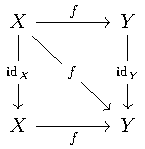
\includegraphics[width=0.6\linewidth]{unit_laws.pdf}
                    \caption{Commutative diagram for Unit Laws}
                    \label{fig: unit_laws}
                \end{minipage} \hspace{0.1\linewidth}
                \begin{minipage}{0.3\linewidth}
                    \centering
                    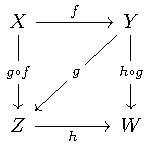
\includegraphics[width=0.6\linewidth]{associativity_law.pdf}
                    \caption{Commutative diagram for Associativity Law}
                    \label{fig: associativity_law}
                \end{minipage}
            \end{figure}

            As examples of commutative diagrams, Figure~\ref{fig: associativity_law} and Figure~\ref{fig: unit_laws} are commutative diagrams for the unit laws and associativity law respectively. 

        
        \subsection{Isomorphism}
        \begin{definition}[Isomorphism]
            Given a category $\mathcal{C}$, a $\mathcal{C}$-morphism $f : X \xrightarrow{\mathcal{C}} Y$ is called an \emph{isomorphism} if there exists a morphism $g : Y \xrightarrow{\mathcal{C}} X$ such that the following diagram commutes:
            \begin{equation}
                \vcenter{\hbox{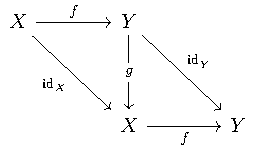
\includegraphics[width=0.3\textwidth]{isomorphism.pdf}}}
                \label{cd: isomorphism}
            \end{equation}
            In other words, $f$ is an isomorphism if there exists a morphism $g$ such that $g \circ f = \textbf{id}_X$ and $f \circ g = \textbf{id}_Y$.

            The morphism $g$ is uniquely determined by $f$ and is called the \emph{inverse} of $f$, denoted as $f^{-1}$.

            Given two objects $X$ and $Y$ in a category $\mathcal{C}$, if there exists an isomorphism from $X$ to $Y$, we say that $X$ and $Y$ are \emph{isomorphic} in $\mathcal{C}$ and write $X \cong Y$.

        \end{definition}

        \subsection{Cartesian closed category}
            \begin{definition}[Terminal object]
                Given a category $\mathcal{C}$, an object $T \in \textbf{obj}(\mathcal{C})$ is called a \emph{terminal object} if for all $X \in \textbf{obj}(\mathcal{C})$, there exists a unique \textbf{C}-morphism $f : X \to T$.
            \end{definition}
            Terminal objects are unique up to isomorphism. In other words, we have the following properties:
            \begin{itemize}
                \item 
                    If $T$ and $T'$ are both terminal objects in $\mathcal{C}$, then there exists a unique isomorphism $f : T \to T'$.
                \item
                    If $T$ is a terminal object in $\mathcal{C}$ and $T \cong T'$, then $T'$ is also a terminal object in $\mathcal{C}$.
            \end{itemize}
            \begin{example}[Terminal object in $\mathcal{Set}$]
                $\mathcal{Set}$ has a terminal object $\{\ast\}$, which is an arbitrary singleton set containing a single element $\ast$.

                For any set $X$, there exists a unique function $f : X \to \{\ast\}$ that maps every element of $X$ to the single element $\ast$ in $\{\ast\}$.
                
                There is a unique isomorphism $f : \{\ast\} \to \{\cdot\}$ for any two singleton sets $\{\ast\}$ and $\{\cdot\}$, which is $f(\ast) = \cdot$.
            \end{example}

            \begin{definition}[Binary product]
                Given a category $\mathcal{C}$, the \emph{binary product} of two objects $X$ and $Y$ in $\mathcal{C}$ is specified by
                \begin{itemize}
                    \item a $\mathcal{C}$-object $X \times Y$;
                    \item two $\mathcal{C}$-morphisms $\pi_1 : X \times Y \to X$ and $\pi_2 : X \times Y \to Y$ called the \emph{projections} of $X \times Y$;
                \end{itemize}
                such that for all $Z \in \textbf{obj}(\mathcal{C})$ and morphisms $f : Z \to X$ and $g : Z \to Y$, there exists a unique morphism $u : Z \to X \times Y$ such that the following diagram commutes in $\mathcal{C}$:
                \begin{equation}
                    \vcenter{\hbox{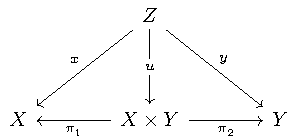
\includegraphics[width=0.4\textwidth]{binary_product.pdf}}}
                    \label{cd: binary_product}
                \end{equation}
                The unique morphism $u$ is written as $\ang{ f, g } : Z \to X \times Y$ where $f = \pi_1 \circ u$ and $g = \pi_2 \circ u$.
            \end{definition}
            It can be shown that the binary product is unique up to (unique) isomorphism.

            \begin{example}[Binary product in $\mathcal{Set}$]
                The binary product of two sets $X$ and $Y$ in $\mathcal{Set}$ is the cartesian product $X \times Y = \{(x,y) \mid x \in X \land y \in Y\}$, where $(x,y)$ are ordered pairs.

                We have the following projections:
                \begin{itemize}
                    \item 
                        $\pi_1 : X \times Y \to X$ is defined as $\pi_1(x,y) = x$ for all $(x,y) \in X \times Y$;
                    \item
                        $\pi_2 : X \times Y \to Y$ is defined as $\pi_2(x,y) = y$ for all $(x,y) \in X \times Y$.
                \end{itemize}

            
                For any set $Z$, for any functions $f : Z \to X$ and $g : Z \to Y$, the unique morphism $u : Z \to X \times Y$ is defined as:
                \[u(z) = (f(z), g(z)) \text{ for all $z \in Z$.}\]
            \end{example}

            \begin{definition}[Exponential]
                Given a category $\mathcal{C}$ with binary products, the \emph{exponential} of two objects $X$ and $Y$ in $\mathcal{C}$ is specified by
                \begin{itemize}
                    \item a $\mathcal{C}$-object $X \Rightarrow Y$;
                    \item a $\mathcal{C}$-morphism $\textbf{app} : (X \Rightarrow Y) \times X \to Y$ called the \emph{application} of $X \Rightarrow Y$;
                \end{itemize}
                such that for all $Z \in \textbf{obj}(\mathcal{C})$ and morphisms $f : Z \times X \to Y$, there exists a unique morphism $u : Z \to X \Rightarrow Y$ such that the following diagram commutes in $\mathcal{C}$:
                \begin{equation}
                    \vcenter{\hbox{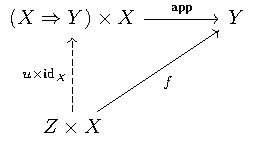
\includegraphics[width=0.4\textwidth]{exponential.pdf}}}
                    \label{cd: exponential}
                \end{equation}
                We write $\textbf{cur} f$ for the unique morphism $u$ such that $f = \textbf{app} \circ (\textbf{cur} f \times \textbf{id}_X)$, 
                where $\textbf{cur} f$ is called the \emph{currying} of $f$.
            \end{definition}
            It can be shown that the exponential is unique up to (unique) isomorphism.

            \begin{example}[Exponential in $\mathcal{Set}$]
                The exponential of two sets $X$ and $Y$ in $\mathcal{Set}$ is the set of all functions from $X$ to $Y$.

                Function application gives the morphism $\textbf{app} : (X \Rightarrow Y) \times X \to Y$ as $\textbf{app}(f,x) = f(x)$ for all $f \in X \Rightarrow Y$ and $x \in X$.

                The currying operation transform a function $f : Z \times X \to Y$ into a function $\textbf{cur} f : Z \to (X \Rightarrow Y)$, which is defined as $\textbf{cur} f(z) = \lambda x.f(z,x)$ for all $z \in Z$ and $x \in X$.
            \end{example}

        \begin{definition}[Cartesian closed category]
            A category $\mathcal{C}$ is called a \emph{cartesian closed category} (CCC) if it has a terminal object, binary products and exponentials of any two objects.
        \end{definition}

        
        \subsection{Functor}
        \begin{definition}[Functor] \label{def: functor}
            Given two categories $\mathcal{C}$ and $\mathcal{D}$, a \emph{functor} $F: \mathcal{C} \to \mathcal{D}$ is specified by
            \begin{itemize}
                \item 
                    a function referred to as object mapping
                    \[\begin{aligned}
                        \textbf{obj}(\mathcal{C}) &\to \textbf{obj}(\mathcal{D}) \\
                        X &\mapsto F(X)
                    \end{aligned}\]

                \item 
                    for each $X, Y \in \textbf{obj}(\mathcal{C})$, a function referred to as functorial mapping
                    \[\begin{aligned}
                        \mathcal{C}{(X,Y)} &\to \mathcal{D}{(F(X),F(Y))} \\
                        f &\mapsto F(f)
                    \end{aligned}\]
            \end{itemize}
            satisfying the following properties:
            \begin{itemize}
                \item 
                    For all $X, Y \in \textbf{obj}(\mathcal{C})$ and $f \in \mathcal{C}{(X,Y)}$, we have: $ F(\textbf{id}_X) = \textbf{id}_{F(X)}$
                \item
                    For all $X, Y, Z \in \textbf{obj}(\mathcal{C})$ and $f \in \mathcal{C}{(X,Y)}$, $g \in \mathcal{C}{(Y,Z)}$, we have: $F(g \circ f) = F(g) \circ F(f)$
            \end{itemize}
        \end{definition}

        
        \subsection{Natural transformation}
        \begin{definition}[Natural transformation]

            Given two categories $\mathcal{C}$ and $\mathcal{D}$, and two functors $F,G: \mathcal{C} \to \mathcal{D}$, a \emph{natural transformation} $\theta : F \to G$ is a family of morphisms $\theta_X \in \mathcal{D}{(F(X),G(X))}$ for each $X \in \textbf{obj}(\mathcal{C})$ such that for all $X, Y \in \textbf{obj}(\mathcal{C})$ and $f \in \mathcal{C}{(X,Y)}$, the following diagram 
            \begin{equation}
                \vcenter{\hbox{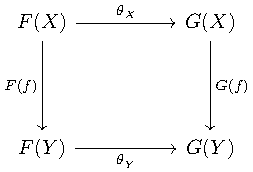
\includegraphics[width=0.3\textwidth]{natural_transformation.pdf}}}
                \label{cd: natural_transformation}
            \end{equation}
            
            commutes in $\mathcal{D}$, i.e. $G(f) \circ \theta_X = \theta_Y \circ F(f)$

        \end{definition}

        
        \subsection{Functor category}
        \begin{definition}[Functor category]
            Given two categories $\mathcal{C}$ and $\mathcal{D}$, the \emph{functor category} $\mathcal{D}^{\mathcal{C}}$ is the category satisfying the following:
            \begin{itemize}
                \item 
                    The objects of $\mathcal{D}^{\mathcal{C}}$ are all functors $\mathcal{C} \to \mathcal{D}$;
                \item 
                    Given two functors $F,G: \mathcal{C} \to \mathcal{D}$, the morphisms from $F$ to $G$ in $\mathcal{D}^{\mathcal{C}}$ are all natural transformations $\theta : F \to G$;
                \item
                    Composition and identity morphisms in $\mathcal{D}^{\mathcal{C}}$ are defined as follows:
                    \begin{itemize}
                        \item 
                            The identity morphism $\textbf{id}_F$ on $F$ is defined as $\theta_X = \textbf{id}_{F(X)}$ for all $X \in \textbf{obj}(\mathcal{C})$;
                        \item
                            The composition of two natural transformations $\theta : F \to G$ and $\phi : G \to H$ is defined as $(\phi \circ \theta)_X = \phi_X \circ \theta_X$ for all $X \in \textbf{obj}(\mathcal{C})$.
                    \end{itemize}
            \end{itemize}
        \end{definition}

        \subsection{Presheaf category}
        A presheaf is a contravariant functor, which means that it reverses the direction of morphisms. In other words, a presheaf is a functor that takes objects in $\mathcal{C}$ and assigns them sets, and takes morphisms in $\mathcal{C}^{\textbf{op}}$ and assigns them functions between the corresponding sets.
        \begin{definition}[Presheaf]
            Given a category $\mathcal{C}$, a \emph{presheaf} on $\mathcal{C}$ is a functor $F: \mathcal{C}^{\textbf{op}} \to \mathcal{Set}$.
            The presheaf $F$ is defined as follows:
            \begin{itemize}
                \item 
                    For each $X \in \textbf{obj}(\mathcal{C})$, $F(X)$ is a set;
                \item
                    For each $X, Y \in \textbf{obj}(\mathcal{C})$ and $f \in \mathcal{C}{(X,Y)}$, $F(f)$ is a function $F(Y) \to F(X)$.
            \end{itemize}
        \end{definition}

        \begin{definition}[Presheaf category]
            Given a category $\mathcal{C}$, the \emph{presheaf category} $\hat{\mathcal{C}}$ is the functor category $\mathcal{Set}^{\mathcal{C}^{\textbf{op}}}$, which explicitly contains the following:
            \begin{itemize}
                \item 
                    The objects of $\hat{\mathcal{C}}$ are all presheaves on $\mathcal{C}$;
                \item
                    Given two presheaves $F,G: \mathcal{C}^{\textbf{op}} \to \mathcal{Set}$, the morphisms from $F$ to $G$ in $\hat{\mathcal{C}}$ are all natural transformations $\theta : F \to G$.
            \end{itemize}
        \end{definition}



        \subsection{Yoneda lemma}
        \begin{definition}[Yoneda functor] \label{def: yoneda}
            Given a category $\mathcal{C}$, the \emph{Yoneda functor} $\yo: \mathcal{C} \to \hat{\mathcal{C}}$ is defined as follows:
            \begin{itemize}
                \item 
                    For each $X \in \textbf{obj}(\mathcal{C})$, $\yo(X)$ is the functor $\mathcal{C}^{\textbf{op}} \to \mathcal{Set}$ defined as:
                    \begin{equation} \label{eq: yoneda_element}
                        \yo(X)(Y) = \mathcal{C}{(Y,X)}
                    \end{equation}
                    for all $Y \in \textbf{obj}(\mathcal{C})$;
                \item
                    For each $X, Y \in \textbf{obj}(\mathcal{C})$ and $f \in \mathcal{C}{(X,Y)}$, $\yo(f)$ is the morphism $\yo(X) \to \yo(Y)$ defined a natural transformation whose component at any given $Z \in \mathcal{C}^{\textbf{op}}$ is given by:
                    \begin{equation} \label{eq: yoneda_morphism}
                        \begin{aligned}
                            (\yo(f))_Z : \mathcal{C}{(Z,Y)} &\to \mathcal{C}{(Z,X)} \\
                            g &\mapsto g \circ f
                        \end{aligned}
                    \end{equation}
                    for all $Z \in \textbf{obj}(\mathcal{C})$.
                \end{itemize}

        \end{definition}

        \begin{theorem}[Yoneda lemma]
            For each small\footnote{See footnote 1.} category $\mathcal{C}$, the \emph{Yoneda lemma} states that for each object $X \in \textbf{obj}(\mathcal{C})$ and each presheaf $F \in \hat{\mathcal{C}}$, there exists a natural isomorphism
            \begin{equation} \label{eq: yoneda_lemma}
                {\hat{\mathcal{C}}}(\yo(X), F) \cong F(X)
            \end{equation}
        \end{theorem}



        \subsection{Cartesian closed structure in presheaf categories} \label{sec: ccc_presheaf}
        \begin{prf}[Cartesian closed structure in presheaf categories]
            Given a small\footnote{See footnote 1.} category $\mathcal{C}$, the presheaf category $\hat{\mathcal{C}}$ is a cartesian closed category.
            \begin{itemize}
                \item 
                    The terminal object in $\hat{\mathcal{C}}$ is the constant functor $\mathbf{1} : \mathcal{C}^{\textbf{op}} \to \mathcal{Set}$, given by 
                    \begin{equation}
                        \begin{cases}
                            \mathbf{1}(X) = \{\ast\} & \text{for all } X \in \textbf{obj}(\mathcal{C}) \\
                            \mathbf{1}(f) = \textbf{id}_{\{\ast\}} & \text{for all } f \in \mathcal{C}{(X,Y)}
                        \end{cases}
                    \end{equation}

                \item
                    The binary product in $\hat{\mathcal{C}}$ is given by the product of functors, which is defined as follows:
                    \begin{equation}
                        \begin{aligned}
                            (F \times G)(X) &= F(X) \times G(X) \\
                            (F \times G)(f) &= F(f) \times G(f)
                        \end{aligned}
                    \end{equation}

                \item
                    The exponential in $\hat{\mathcal{C}}$ is derived from the Yoneda lemma,
                    \begin{equation}
                        \begin{aligned}
                            G^{F}(X) &= \hat{\mathcal{C}}(\yo(X) \times F, G) \\
                            G^{F}(f)(\theta) &= \theta \circ (\yo(f) \times \textbf{id}_F) \quad \text{for all } \theta \in \hat{\mathcal{C}}(\yo(Y) \times F, G)
                        \end{aligned}
                    \end{equation}
            \end{itemize}
        \end{prf}
                
        \subsection{Curry-Howard-Lambek correspondence} \label{subsec: curry-howard-lambek}
        Joachim Lambek showed that cartesian closed categories provide a natural semantic setting for the simply typed lambda calculus (STLC)~\autocite{lambek}. His work builds upon Curry-Howard correspondence~\autocite{curry-howard}, the isomorphism between logic and type theory, where propositions correspond to types and proofs correspond to terms. The Curry-Howard-Lambek correspondence can be summarised as follows:
        \begin{table}[H]
            \centering
            \begin{tabular}{|c|c|c|}
                \hline
                \textbf{Logic} & \textbf{Type theory} & \textbf{Category theory} \\
                \hhline{|=|=|=|}
                Proposition & Type & Object \\
                \hline
                Proof & Term & Morphism \\
                \hline
                Falsity & Empty type & Initial object \\
                \hline
                Truth & Unit type & Terminal object \\
                \hline
                Implication & Function type & Exponential \\
                \hline
                Conjunction & Product type & Product \\
                \hline
                Disjunction & Sum type & Coproduct \\
                % Universal quantification & Dependent product type &  \\
                % Existential quantification & Dependent sum type &  \\
                \hline
            \end{tabular}
            \caption{Curry-Howard-Lambek correspondence}
            \label{tab: curry-howard-lambek}
        \end{table}
        This correspondence forms the foundation of functional programming languages that can be used to implement proofs. 

    \section{Agda}
        \subsection{Basic data types and pattern matching}
        Here is a simple example selected from PLFA~\autocite{plfa} to illustrate the basic data types and pattern matching in Agda. The example is a definition of natural numbers and a plus function.

        \[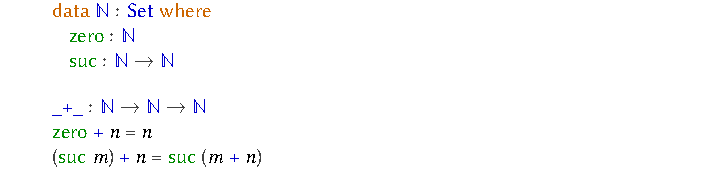
\includegraphics[scale=1.2]{natural_plus.pdf}\]

        In Agda we use the $\og{\mathsf{data}}$ keyword to define a type. Every type has a type, and we use $\mb{\mathsf{Set}}$ to denote the type of all small types. To define a type, we specify its type and its constructors. To define a function, we specify its type and pattern match the input according to the constructors of the type.

        \subsection{Dependent Types}
        A dependent type is a type that depends on a value. In terms of type judgement, simple types are in form of
        \[ x_1 : T_1, x_2 : T_2, \dots, x_n : T_n \vdash t(x_1, \dots, x_n) : T \]
        In contrast, dependent types are in form of
        \[ x_1 : T_1, x_2 : T_2, \dots, x_n : T_n \vdash t(x_1, \dots, x_n) : T(x_1, \dots, x_n) \]
        or more generally
        \[ x_1 : T_1, x_2 : T_2(x_1), \dots, x_n : T_n(x_1, \dots, x_{n-1}) \vdash t(x_1, \dots, x_n) : T(x_1, \dots, x_n) \]

        A classical example of dependent types in Agda is the type of vectors, which are lists with a length. 

        \[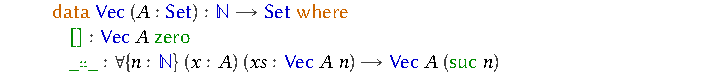
\includegraphics[scale=1.2]{vector.pdf}\]

        Here a data type $\mb{\mathsf{Vec}}$ is defined for vectors. The type of vectors is dependent on the length of the vector. With dependent types, we can encode properties directly into types.

        \subsection{Equality, congruence and substitution}\label{subsec: equality}
        Equality here refers to the propositional equality. In Agda it is defined as
        \[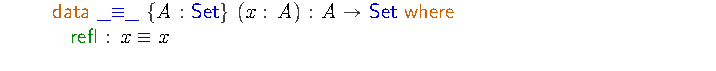
\includegraphics[scale=1.2]{equality.pdf}\]
        With equality as a type, whenever we want to prove that two terms are equal, we need to provide a witness of the equality. For example if we want to prove $x \equiv y$, we write out a term of type \textit{x} \mb{\textsf{≡}} \textit{y}, and then give its definition, which constructs a proof of the equality. All of the examples here are type-checked by Agda, so they are all valid proofs. 
        
        Two simple proofs that directly use the definition of equality is as follows:
        \[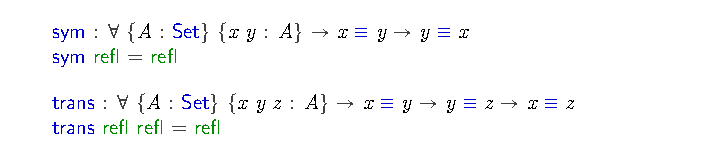
\includegraphics[scale=1.2]{sym_trans.pdf}\]
        Here \textit{y} and \textit{z} are reduced to \textit{x} by the definition of the constructor \gn{\textsf{refl}}. The properties are called \emph{symmetry} and \emph{transitivity} of equality, which are very useful for later proofs.

        We can also have more complex proof with \emph{congruence} and \emph{substitution}, which can also be directly derived from the definition of equality as follows:
        \[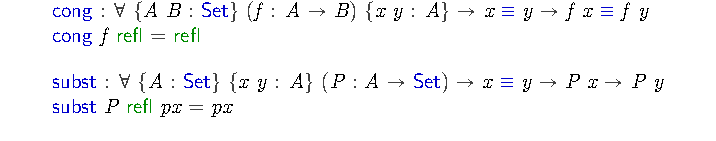
\includegraphics[scale=1.2]{cong_subst.pdf}\]
        % \emph{Congruence} is a property of equality that states that if two terms are equal, then they can be substituted for each other in any context. \emph{Substitution} is a property where we can get a new proof by replacing a term in a proof with another term that is equal to it. 

        Here is a simple example of how congruence can be used in a proof:
        \[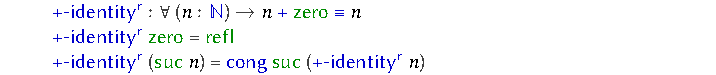
\includegraphics[scale=1.2]{plus_right_identity.pdf}\]
        In this example, we want to prove that \gnt{zero} is the right identity of the plus function. This property cannot be directly shown by using \gn{\textsf{refl}} because \gn{\textsf{refl}} only knows about definitional equality. In the definition of the plus function, only the first argument is pattern matched, so we can only show that \gnt{zero} is the left identity of the plus function by directly sing the \gn{\textsf{refl}}. To show that \gnt{zero} is the right identity of the plus function, we need to do an inductive proof by pattern matching on the first argument of the plus function. 
        
        In the base case, we have \gnt{zero} \mb{+} \gnt{zero} \mb{≡} \gnt{zero}, which is true by the definition of the plus function.
        
        In the inductive case, we need to show \gnt{suc} \textit{n} \mb{+} \gnt{zero} \mb{≡} \gnt{suc} \textit{n}. The left hand side is definitionally equal to \gnt{suc} (\textit{n} \mb{+} \gnt{zero}). By the inductive hypothesis, we know that \textit{n} \mb{+} \gnt{zero} \mb{≡} \textit{n}, so we can substitute \textit{n} for \textit{n} \mb{+} \gnt{zero} in the right-hand side by congruence, and we are done.

        % \subsection{With and Rewrite}

        \subsection{Standard library} \label{subsec: stdlib}
        The Agda standard library~\autocite{agda_std} is a collection of modules that provide a wide range of useful functions and types. It includes modules for basic data types, such as natural numbers, lists, and vectors. In my implementation, standard library is used as a reference for defining a customised library, which is specified in~\secref{sec: lib}.

        \subsubsection{Builtin pragma} \label{subsubsec: builtin_pragma}
        With standard library, we can use literal natural numbers \ppt{1}, \ppt{2}, \dots\ instead of calling the constructor \gnt{suc} multiple times. This feature can be extended to self-defined functions with a \og{\textsf{BUILTIN}} pragma. We simply add the following two lines after the definition of \mb{\bN} and \mb{\_+\_}: 
        \[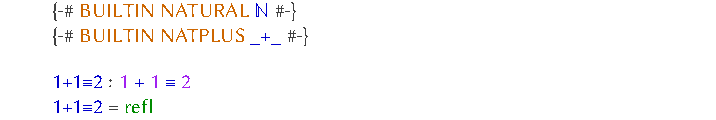
\includegraphics[scale=1.2]{natural_pragma.pdf}\]
        Note that in agda we can use unicode characters for names of terms, which makes the code more readable. For example, here we simply name the term \mb{\textsf{1+1≡2}}.

        
        \subsection{Interactive programming with holes} \label{subsec: holes}
        A feature of Agda is interactive programming with holes. When users leave holes in place of undefined terms, Agda's type checker will infer the type of the hole, show available variables and candidate terms with their types. Holes also supports case split and refinement, which means we can fill in a hole partially and split it into smaller holes. This feature is used in my implementation. The complex terms are incrementally filled and verified by refining partial implementations, reducing post-hoc debugging and ensuring robustness.


    \section{Requirement Analysis}
    To complete the compiler in Agda I need to implement the following components:
    \begin{itemize}
        \item 
            A file \texttt{source.agda} that record the syntax of the source language, which include basic instructions in STLC with store.

        \item
            A file \texttt{target.agda} that record the syntax of the target language.

        \item
            A file \texttt{compiler.agda} that uses \texttt{source.agda} and \texttt{target.agda}, and write functions whose input is a closed term in the source language and output is a term in the target language.
        \item 
            A file \texttt{test.agda} that contains test cases for the compiler. The test cases are written in the source language, and the expected output is written in the target language. 
    \end{itemize}
    The implementation and type-checking of all files specified above constitutes a necessary and sufficient condition for meeting the project's success criteria mentioned in~\secref{sec: contributions}.

\chapter{Implementation} \label{chap: implementation}
    \minitoc
    This chapter details the implementation of the compiler in Agda. Following a brief overview of the tools used~(\secref{sec: tools}), it provides a repository overview~(\secref{sec: repo_overview}). Then it discusses the intrinsic syntax of the source language~(\secref{sec: source}) and the grammar of target language~(\secref{sec: target}), leading to the problem of implementing a proof-relevant natural number subtraction.

    To address this, it presents the customised library~(\secref{sec: lib}) with two different approaches for implementing subtraction: one using additional proof object and the other using Fin, a dependent type. It compares the two approaches and discusses the trade-offs between them. The chapter concludes with a detailed implementation of the compiler~(\secref{sec: compiler}).
    

    \section{Tools used} \label{sec: tools}
    The project is implemented in Agda 2.7.0.1, the latest stable version at the time of writing.

    Completing the project is an iterative process. I used Git~\autocite{git} for version control, and work had been synchronised with a GitHub~\autocite{github} repository for backup.

    For the development environment, I tried both Emacs~\autocite{emacs} and Visual Studio Code~\autocite{vscode} with an agda-mode extension~\autocite{agda_mode} on Windows Subsystem for Linux with Ubuntu~\autocite{wsl_ubuntu} 22.04 LTS. I am more familiar with the snippet and syntax highlighting features of Visual Studio Code, so I used it for most of the development. 

    Code from the PLFA tutorial and Agda standard library~\autocite{agda_std} were used as references for implementation of the source language and the customised library. Apart from that, the code is written from scratch.

    \section{Repository Overview} \label{sec: repo_overview}
        \subsection{Directory structure}
        The repository contains two independent implementations of the compiler, organised in two directories: \texttt{fin} and \texttt{proof} as follows:
        \dirtree{%
            .1 ..
            .2 fin.
            .3 lib.agda.
            .3 source.agda.
            .3 target.agda.
            .3 compiler.agda.
            .3 test.agda.
            .2 proof.
            .3 lib.agda.
            .3 source.agda.
            .3 target.agda.
            .3 compiler.agda.
            .3 test.agda.
        }

        \subsection{File dependencies and descriptions}
        The dependency graph for each implementation is identical as follows:
        \begin{figure}[H]
            \centering
            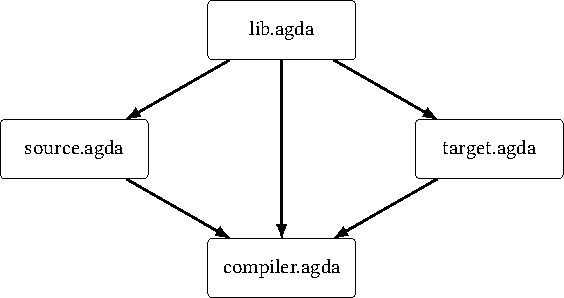
\includegraphics[width=0.6\textwidth]{dependencies.pdf}
            \caption{Dependency graph for the compiler}
            \label{fig: dependencies}
        \end{figure}

        \begin{table}[H]
            \centering
            \begin{tabular}{|l|l|l|}
                \hline
                \textbf{File} & \textbf{Description}\\
                \hhline{|=|=|}
                \texttt{lib.agda} & shared utilities (e.g. natural numbers and operations, equality, etc.) \\
                \hline
                \texttt{source.agda} & source language syntax \\
                \hline
                \texttt{target.agda} & target language (stack machine) instructions \\
                \hline
                \texttt{compiler.agda} & compiler derived from denotational semantics \\
                \hline
                \texttt{test.agda} & test cases for the compiler \\
                \hline
            \end{tabular}
            \caption{File descriptions}
            \label{tab: file_descriptions}
        \end{table}

    \section{Source Language} \label{sec: source}
    % A simply typed lambda calculus (STLC) is a typed lambda calculus with only one type constructor ($\Rightarrow$) \footnote{Normally we use $\to$ to denote the function type, but here we use $\Rightarrow$ to be consistent with the notation in Agda, as $\to$ is a primitive in Agda.} that builds function types. 
    The source language is a simply typed lambda calculus (STLC) with store, following the syntax in Reynolds' paper~\autocite{Reynolds}.
        \subsection{Types}
        The source language has four primitive types:
        \begin{itemize}
            \item 
                \textsf{comm}: commands, which is the type of programs
            \item 
                \textsf{intexp}: integer expressions, corresponding to \texttt{int} in most programming languages
            \item 
                \textsf{intacc}: integer acceptors, representing reference to integer values
            \item 
                \textsf{intvar}: integer variables, which are integer acceptors that can also be used as expressions with automatic dereferencing
        \end{itemize}
        and general types are defined as follows: 
        \[ A, B := \textsf{comm} \mid \textsf{intexp} \mid \textsf{intacc} \mid \textsf{intvar} \mid A \Rightarrow B \] 
        which corresponds with the following agda implementation:
        \[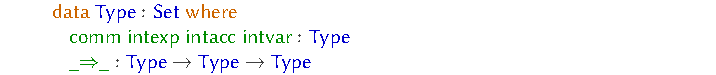
\includegraphics[scale=1.2]{/source/types.pdf}\]

        \subsubsection{Subtypes}
        I use the preorder $A ≤: B$ to denote the subtype relation $A$ is a subtype of $B$, as it has the following properties:
        \begin{figure}[H]
            \centering
            \includegraphics[width=0.5\textwidth]{subtype.pdf}
            \caption{Preorder of subtypes}
            \label{fig: subtype}
        \end{figure}

        The source language has the following subtype relations:
        \[ \textsf{intvar} \leq: \textsf{intexp} \qquad \textsf{intvar} \leq: \textsf{intacc} \]
        since a variable can be used as an expression (e.g. $\mathsf{x} + 1$) or an acceptor (e.g. $\mathsf{x} := 1$).

        For function types we have the contravariant subtyping:
        \begin{figure}[H]
            \centering
            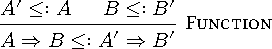
\includegraphics[width=0.3\textwidth]{subtype_function.pdf}
            \caption{Contravariant subtyping for function types}
            \label{fig: subtype_fun}
        \end{figure}
        
        it is defined in Agda as follows:
        \[\includegraphics[scale=1.2]{/source/subtype.pdf}\]

        \subsection{Contexts and variables}
        We define the context as a finite list of types as follows:
        \[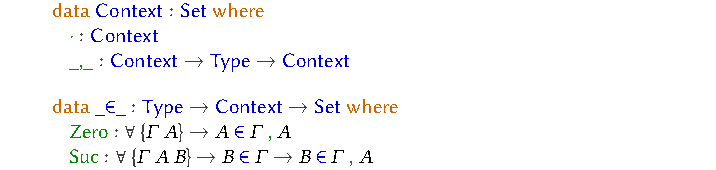
\includegraphics[scale=1.2]{/source/contexts.pdf}\]
        When we are looking for a variable, \gnt{Zero} case corresponds to the situation where the variable is the head of the context, and the \gnt{Suc} case corresponds to the situation where the variable is in the tail of the context. The number formed by \gnt{Zero} and \gnt{Suc} is the index of the variable in the context, called the \emph{de Bruijn index}~\autocite{de_bruijn}. 


        \subsection{Terms and the typing judgement} \label{subsec: terms}
        The terms are defined as follows:
        \[\begin{aligned}
            c_1, c_2 &= \texttt{skip} \mid c_1; c_2 \mid a := e \mid \texttt{new } x \texttt{ in } c_1 \\
            e_1, e_2 &= \texttt{lit } z \mid -e_1 \mid e_1 + e_2 \mid \lambda e_1.\ e_2 \mid e_1\ e_2 \mid x \\
        \end{aligned}\]
        
        and the typing judgement are described in the following rules:
        \begin{figure}[H]
            \centering
            \begin{minipage}{0.4\textwidth}
                \centering
                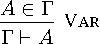
\includegraphics{source_terms_var.pdf}
                \caption{Variable typing rule}
                \label{fig: rule_var}
            \end{minipage} \hspace{0.1\textwidth}
            \begin{minipage}{0.4\textwidth}
                \centering
                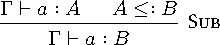
\includegraphics{source_terms_subtype.pdf}
                \caption{Subtyping rule}
                \label{fig: rule_subtype}
            \end{minipage}
        \end{figure}
        \begin{figure}[H]
            \centering
            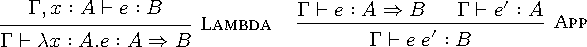
\includegraphics{source_terms_lambda.pdf}
            \caption{Lambda abstraction typing rules}
            \label{fig: rule_lambda}
        \end{figure}
        \begin{figure}[H]
            \centering
            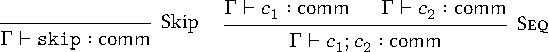
\includegraphics{source_terms_comm_1.pdf}
            \caption{Command typing rules (part 1)}
            \label{fig: rule_comm_1}
        \end{figure}
        \begin{figure}[H]
            \centering
            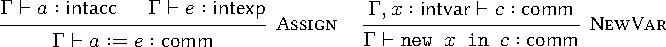
\includegraphics{source_terms_comm_2.pdf}
            \caption{Command typing rules (part 2)}
            \label{fig: rule_comm_2}
        \end{figure}
        \begin{figure}[H]
            \centering
            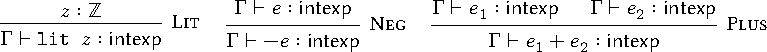
\includegraphics{source_terms_intexp.pdf}
            \caption{Integer expression typing rules}
            \label{fig: rule_intexp}
        \end{figure}

        The corresponding Agda implementation is as follows, note that the Agda implementation only does not include the name of the terms, as a term can be specified by how it is constructed (i.e. the name of the typing rules and the corresponding types)
        \[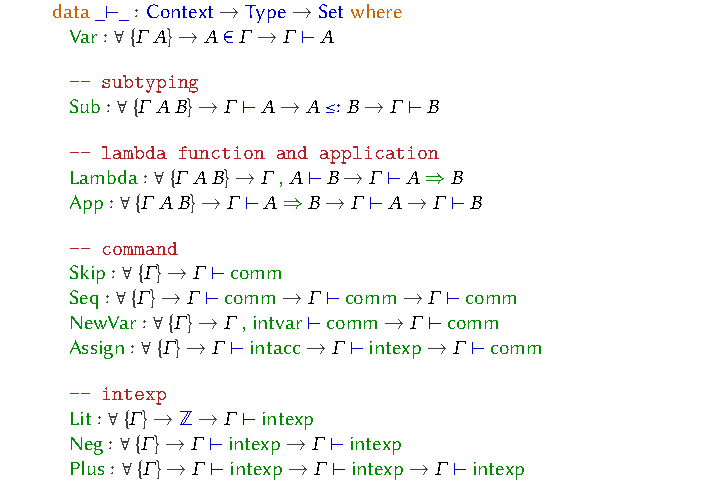
\includegraphics[scale=1.2]{/source/terms.pdf}\]

        \subsection{Operational Semantics}
        The operational semantics of the source language is defined with renaming, substitution and reduction rules. However, since the compiler itself does not require the operational semantics, the implementation is included in Appendix~\ref{app: operational_semantics}. Operational semantics can be used to verify the correctness of the compiler in the future, but it is beyond the scope of this project.


    \section{Target Language} \label{sec: target}
    The target language is an assembly-style intermediate language for a stack machine. It is defined with four stack-descriptor-indexed families of non-terminals: 
    \begin{itemize}
        \item 
            $\bracket{\textsf{L}_{\textit{sd}}}$: left-hand sides
        \item 
            $\bracket{\textsf{S}_{\textit{sd}}}$: simple right-hand sides
        \item
            $\bracket{\textsf{R}_{\textit{sd}}}$: right-hand sides
        \item
            $\bracket{\textsf{I}_{\textit{sd}}}$: instruction sequences
    \end{itemize}
    The intent of the indexing here is any instructions with the form $\bracket{\textsf{I}_{\textit{sd}}}$ is an instruction sequence that can be executed when the current stack descriptor is $\textit{sd}$. 

    The following subsections start with the definition of stack descriptors, then define the grammar of the target language, and finally discuss the problem of subtraction of natural numbers.

    \subsection{Stack descriptor}
    Now, I define the stack descriptor in Agda, as well as their pre-order, operations (addition and subtraction), and properties about ordering.

    The stack descriptor $\textit{sd}$ is defined as a pair of natural numbers $\ang{f, d}$, where $f$ is the frame number and $d$ is the displacement. 

    It is defined in Agda as follows:
    \[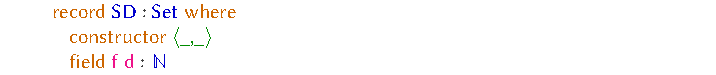
\includegraphics[scale=1.2]{/target/stack_descriptor.pdf}\]

    For a stack descriptor $\textit{sd}$, we can use \dpink{SD.f} $\textit{sd}$ to access the frame number and \dpink{SD.d} $\textit{sd}$ to access the displacement. 

    \subsubsection{Order}
    The stack descriptor is ordered lexicographically with $\leq_\mathsf{s}$ as follows:
    \[\ang{f, d} \leq_\mathsf{s} \ang{f', d'} \Leftrightarrow f < f' \lor (f = f' \land d \leq d')\]

    It is defined in Agda as follows:
    \[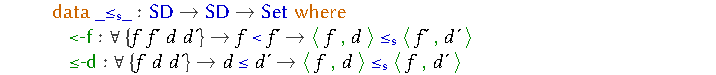
\includegraphics[scale=1.2]{/target/stack_descriptor_order.pdf}\]

    \subsubsection{Addition and subtraction of stack descriptors}
    The addition and subtraction of stack descriptors is defined as follows:
    \[\ang{f, d} \pm_\mathsf{s} n = \ang{f, d \pm n} \text{ for } n \in \mathbb{N}\]
    Addition of stack displacement is defined in Agda as follows:
    \[
\includegraphics[scale=1.2]{/target/stack_descriptor_add.pdf}\]
    For subtraction, we need to make sure that the subtraction is valid, i.e. $\ang{f, d} -\mathsf{s} n$ is only defined for $n \leq d$. This leads us to the problem of defining the subtraction of natural numbers, which is explained in detail in~\secref{subsec: subtraction}.

    \subsubsection{Properties}
    The properties of stack descriptors can be summarised as follows:
    \begin{table}[H]
        \centering
        \begin{tabular}{|c|c|}
            \hline
            \textbf{Agda term} & \textbf{Mathematical meaning} \\
            \hhline{|=|=|}
            \mbt{≤ₛ-refl} & $\forall sd.\ sd \leq_\mathsf{s} sd$ \\
            \hline
            \mbt{≤ₛ-trans} & $\forall sd, sd', sd''.\ sd \leq_\mathsf{s} sd' \land sd' \leq_\mathsf{s} sd'' \Rightarrow sd \leq_\mathsf{s} sd''$ \\
            \hline
            \mbt{+ₛ→≤ₛ} & $\forall sd, n.\ sd \leq_\mathsf{s} sd +_\mathsf{s} n$ \\
            \hline
            \mbt{sub-sd≤ₛ} & $\forall sd, sd', sd''. sd' \equiv sd'' \land sd \leq_\mathsf{s} sd' \Rightarrow sd \leq_\mathsf{s} sd''$ \\
            \hline
            \mbt{–ₛ≡} & $\forall f, d, d′, n.\ d′ - n \equiv d \Rightarrow \ang{f, d} \equiv \ang{f, d′} -_\mathsf{s} n$ \\
            \hline
        \end{tabular}
        \caption{Properties of order and addition of stack descriptors}
        \label{tab: stack_descriptor_properties}
    \end{table}
    % We can use reflexivity and transitivity of the order $<$ and $\leq$ to prove that the order of stack descriptors $\leq_\mathsf{s}$ is a preorder. The proof in Agda is as follows:
    % \begin{proof}
    %     We need to show that $\leq_\mathsf{s}$ is reflexive and transitive. 
    %     \begin{itemize}
    %         \item 
    %             Reflexivity: $\textit{sd} \leq_\mathsf{s} \textit{sd}$ is trivially true since $f = f$ and $d \leq d$.
    %         \item
    %             Transitivity: if $\ang{f, d} \leq_\mathsf{s} \ang{f', d'}$ and $\ang{f', d'} \leq_\mathsf{s} \ang{f'', d''}$, we do the following case split:
    %             \begin{enumerate}
    %                 \item 
    %                     If $f < f'$, $f' = f''$ and $d \leq d'$, then $f < f''$; 
    %                 \item 
    %                     If $f < f'$ and $f' < f''$, then $f < f''$ by transitivity of $<$;
    %                 \item
    %                     If $f = f'$, $d \leq d'$ and $f' < f''$, then $f < f''$;
    %                 \item
    %                     Otherwise $f = f''$ and $d \leq d''$ by transitivity of $\leq$. \footnote{Note that the properties of $=$ is not required in as in the Agda definition of $\leq_\mathsf{s}$, we directly define $f'$ to be $f$ instead of defining a equivalence relation, thus equivalence can be checked directly via type checking.}
    %             \end{enumerate}
    %     \end{itemize}
    % \end{proof}

    % The proof is defined in Agda as follows:
    % \[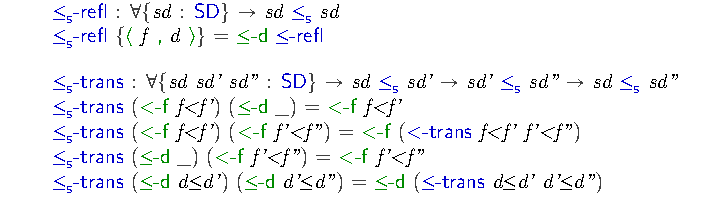
\includegraphics[scale=1.2]{/target/stack_descriptor_order_proof.pdf}\]

    % When a natural number is added to a stack descriptor, it is guaranteed that the new stack descriptor is not less than the old stack descriptor. This can be proved directly using the same properties of integer addition. The proof is defined in Agda as follows:
    % \[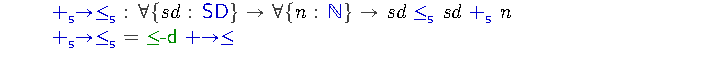
\includegraphics[scale=1.2]{/target/stack_descriptor_add_proof.pdf}\]

    \subsection{Grammar} \label{subsec: grammar}
    The grammar of the target language\footnote{This grammar can be extended with subroutines as an \textsf{L} command, and conditionals as an \textsf{I} command} is defined as follows, given the current stack descriptor $\textit{sd} = \ang{f, d}$, and new stack descriptor $\textit{sd′}$ and $\textit{sd\textsuperscript{v}}$:
    \begin{figure}[H]
        \centering
        \[\begin{aligned}
            \bracket{\textsf{L}_{\textit{sd}}} ::={}& \textit{sd\textsuperscript{v}} \quad \text{when } \textit{sd\textsuperscript{v}} \leq_\mathsf{s} \textit{sd} \\
                            % &\mid \texttt{sbrs}  \\
            \bracket{\textsf{S}_{\textit{sd}}} ::={}& \bracket{\textsf{L}_{\textit{sd}}} \\
                            &\mid \texttt{lit } \bracket{\text{integer}} \\
            \bracket{\textsf{R}_{\textit{sd}}} ::={}& \bracket{\textsf{S}_{\textit{sd}}} \\
                            &\mid \bracket{ \text{unary operator} } \bracket{ \textsf{S}_{\textit{sd}}}\\
                            &\mid \bracket{\textsf{S}_{\textit{sd}}} \bracket{\textsf{binary operator}} \bracket{ \textsf{S}_{\textit{sd}} } \\
            \bracket{\textsf{I}_{\textit{sd}}} ::={}& \texttt{stop} \\
                            &\left.
                            \begin{aligned}
                            &|{\ } \bracket{\textsf{L}_{\textit{sd}+\delta}} := \bracket{\textsf{R}_{\textit{sd}}}[\delta] \text{ ; } \bracket{\textsf{I}_{\textit{sd}+\delta}} \\
                            % &|{\ } \texttt{if } \bracket{\textsf{S}_{\textit{sd}}} \bracket{\text{relational operator}} \bracket{\textsf{S}_{\textit{sd}}}[\delta] \\
                            % & \hphantom{\mid {}} \texttt{ then } \bracket{\textsf{I}_{\textit{sd}+\delta}} \texttt{ else } \bracket{\textsf{I}_{\textit{sd}+\delta}} \\
                            &|{\ } \texttt{adjustdisp} [\delta] \text{ ; } \bracket{\textsf{I}_{\textit{sd}+\delta}} \\
                            \end{aligned}
                            \quad \right\} \text{if } d + \delta \geq 0  \\
                            &{}\mid{} \texttt{popto } \textit{sd′} \text{ ; } \bracket{\textsf{I}_{\textit{sd′}}} \quad \text{when } \textit{sd′} \leq_\mathsf{s} \textit{sd} \\
        \end{aligned}\]
        \caption{Target language grammar}
        \label{fig: target_grammar}
    \end{figure}
    Some explanations of the grammar are as follows:
    \begin{itemize}
        % \item 
        %     $\texttt{sbrs}$: a register used to communicate the result of function procedures implemented by closed subroutines.
        \item 
            $\texttt{lit}$: a literal integer.
        \item 
            $\texttt{stop}$: stops the execution of the program.
        \item 
            $\delta$: an integer representing the displacement adjustment.
        \item 
            $\texttt{adjustdisp}$: adjusts the displacement of specified stack descriptor.
        \item 
            $\texttt{popto}$: pops to the specified stack descriptor, which is used to reduce the number of frames.
    \end{itemize}
    Note that the design of right-hand sides ensures that the right operand of the assignment contains at most one operator, which means that any instruction that involves multiple operators must be divided into multiple instructions. This feature of the target language significantly complicates the compilation of integer expressions, which we will analysis in detail in~\secref{subsubsec: compiler_intexp}.

    A fundamental property of the target language is its order-preserving extension with respect to stack descriptors: any term operating on a smaller stack descriptor can be systematically lifted to operate on a larger one. As later formalised in~\secref{subsec: functorial_mapping}, this property exhibits a functorial nature, and is essential for the construction of the compiler.

    % \subsubsection{Operators}
    The operators are defined as follows:
    \[\begin{aligned}
        \textsf{unary operator} &\in \{\texttt{UNeg}\} \\
        \textsf{binary operator} &\in \{\texttt{BPlus}, \texttt{BMinus}, \texttt{BTimes}\} \\
        % \textsf{relational operator} &\in \{\texttt{RLeq}, \texttt{RLt}\}
    \end{aligned}\]

    The operators are defined in Agda as follows:
    \[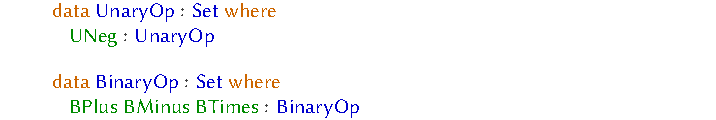
\includegraphics[scale=1.2]{/target/operators.pdf}\]

    % \subsubsection{Left-hand sides, simple right-hand sides and right-hand sides}
    The left-hand sides, simple right-hand sides and right-hand sides are straightforward, and they are defined as follows in Agda:
    \[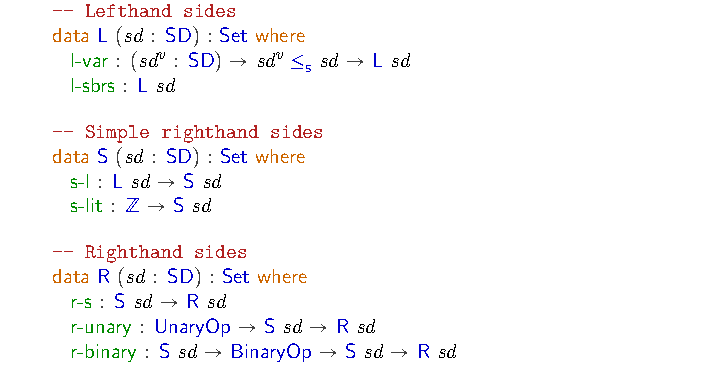
\includegraphics[scale=1.2]{/target/leftrighthand_sides.pdf}\]

    % \subsubsection{Instruction sequences}
    In the instruction sequences, $\delta$ as a displacement adjustment can be positive, zero or negative. To make a rigorous definition, I define $\delta$ as a natural number, and treat the positive and negative displacements as two different instructions, using addition and subtraction of stack descriptors respectively. 

    The assignment with negative displacement is left to discuss in~\secref{subsec: subtraction}, since it involves proof objects to validate the subtraction. 
    The remaining instruction sequences are defined in Agda as follows:
    \[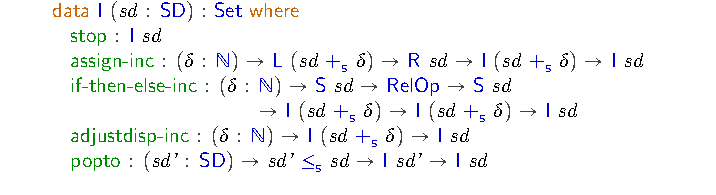
\includegraphics[scale=1.2]{/target/instruction_inc.pdf}\]


    \section{Customised Library} \label{sec: lib}
    The customised library is a collection of types and functions centred around natural numbers, their operations and properties. Instead of using the standard library~\autocite{agda_std}, I implemented a customised library for the following reasons:
    \begin{itemize}
        \item
            \textbf{Specialised Requirements}: The standard library's definitions (e.g. subtraction as monus, `$\dotdiv$') do not align with my project's need for a rigorously defined subtraction operation. This is specified in~\secref{subsec: subtraction}.
        \item
            \textbf{Verification Clarity}: By defining the basic data types and functions from scratch, I can tailor properties (e.g. the property `$n-[n-m] \equiv m$') to my specific requirements, and avoid unnecessary complexity (e.g. `$\leq$' being also defined as a boolean predicate in the standard library). 
        \item
            \textbf{Minimal Dependencies}: Avoiding the standard library reduces external assumptions, making the project self-contained. 
    \end{itemize}
    All definitions and properties can be found in Appendix~[TBD].

    \subsection{Definitions from standard library}
    The following is a list of definitions (or their variants) from the standard library and PLFA~\cite{plfa} that are redefined in the customised library:
    \begin{itemize}
        \item 
            Natural numbers ($\mb{\bN}$), integers ($\mb{\bZ}$) and addition (\mbt{+}).
        \item
            Equality (\mbt{≡}), congruence ($\mb{\mathsf{cong}}$), substitution ($\mb{\mathsf{sub}}$) and transitivity of equality ($\mb{\mathsf{trans}}$).
        \item
            Order of natural numbers, including \mbt{≤} and \mbt{<}.
        \item
            Properties of preorder and addition (summarised in Table~\ref{tab: properties}).
    \end{itemize}
    \begin{table}[H]
        \centering
        \begin{tabular}{|l|l|}
            \hline
            \textbf{Agda term} & \textbf{Mathematical meaning} \\
            \hhline{|=|=|}
            \mbt{+-identity\textsuperscript{r}} & $\forall n \in \bN.\ n + 0 = n$ \\
            \hline
            \mbt{+-suc\textsuperscript{r}}& $\forall m, n \in \bN.\ m + \textsf{suc } n = \textsf{suc } (m + n)$ \\
            \hline
            \mbt{+-comm\textsuperscript{r}} & $\forall m, n \in \bN.\ m + n \equiv n + m$ \\
            \hline
            \mbt{≤-irrelevant} & For all $m, n \in \bN$, we consider all proofs of $m \leq n$ to be equal. \\
            \hline
            \mbt{≤-refl} & $\forall n \in \bN.\ n \leq n$ \\
            \hline
            \mbt{≤-trans} & $\forall m, n, p \in \bN.\ m \leq n \land n \leq p \Rightarrow m \leq p$ \\
            \hline
            \mbt{n≤suc-n} & $\forall n \in \bN.\ n \leq \textsf{suc } n$ \\
            \hline
            \mbt{m≡n,p≤n}\mb{$\to$}\mbt{p≤m} & $\forall p, m, n \in \bN.\ m \equiv n \land p \leq n \Rightarrow p \leq m$ \\
            \hline
            \mbt{+}\mb{$\to$}\mbt{≤} & $\forall m, n \in \bN.\ m \leq m + n$ \\
            \hline
            \mbt{+}\mb{$\to$}\mb{≤\textsuperscript{r}} & $\forall m, n \in \bN.\ m \leq n + m$ \\
            \hline
            \mbt{<-trans} & $\forall m, n, p \in \bN.\ m < n \land n < p \Rightarrow m < p$ \\
            \hline
            \mbt{<}\mb{$\to$}\mbt{s≤} & $\forall m, n \in \bN.\ m < n \Rightarrow \textsf{suc } m \leq n$ \\
            \hline
            \mbt{<}\mb{$\to$}\mbt{≤} & $\forall m, n \in \bN.\ m < n \Rightarrow m \leq n$ \\
            \hline
            \mbt{≤-compare} & $\forall m, n \in \bN.\ m \leq n \lor n \leq m$ \\
            \hline
        \end{tabular}
        \caption{Properties of order and addition}
        \label{tab: properties}
    \end{table}

    % \subsection{Natural numbers, integers and addition} \label{subsec: natural_numbers}
    % The definition of natural numbers, integers and addition is standard, and it is defined as follows:
    % \[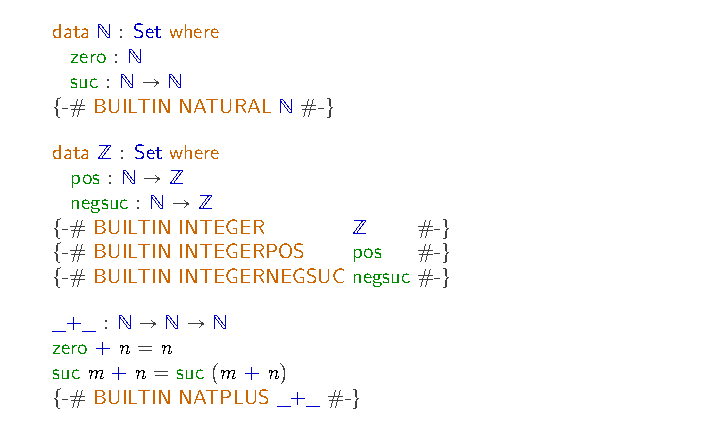
\includegraphics[scale=1.2]{/lib/natural.pdf}\]
    % The use of \og{\textsf{BUILTIN}} is specified in~\secref{subsubsec: builtin_pragma}.

    % \subsection{Equality, congruence and substitution}
    % The definition of equality, congruence and substitution is similar to the one in~\secref{subsec: equality}.\footnote{The definition of equality and related properties in the custom library differ slightly by using an indexed $\mb{\mathsf{Set}}$, which provides a more general formulation. See Appendix [corresponding link].}

    % \subsection{Order of natural numbers} \label{subsec: order}
    % The order of natural numbers we defined include $\leq$ and $<$, we use a simplified definition compared to the one in the standard library as follows:
    % \[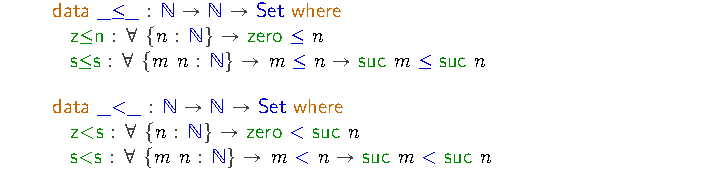
\includegraphics[scale=1.2]{/lib/order.pdf}\]

    % \subsection{Properties of order and addition}
    % \subsubsection{Transitivity and reflexivity}
    % The transitivity and reflexivity of the order $<$ and $\leq$ are defined as follows:
    % \[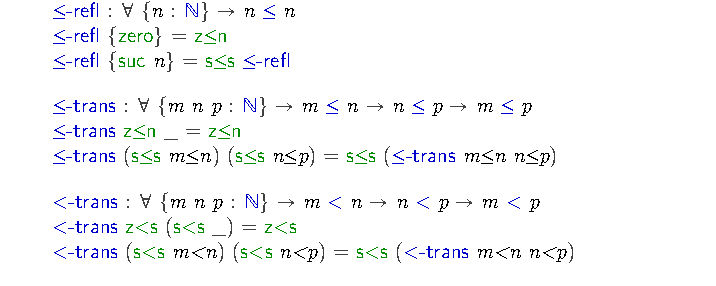
\includegraphics[scale=1.2]{/lib/order_proof.pdf}\]

    % \subsubsection{Implication of order}
    % We know that $\forall m, n \in \bN$, if $m < n$, then we have $m + 1 \leq n$ and $m \leq n$. This is defined in Agda as follows:
    % \[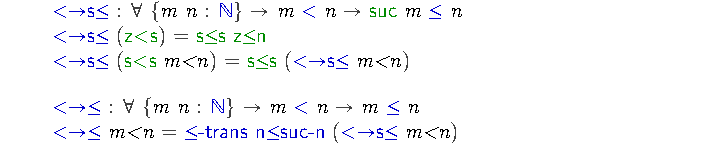
\includegraphics[scale=1.2]{/lib/order_implication.pdf}\]

    % \subsubsection{Totality of order} \label{subsubsec: order_totality}
    % It is useful to case split the order of natural numbers, i.e. for any $m, n \in \bN$, we have $m \leq n$ or $n \leq m$. This is defined in Agda by defining either case as an instance of the \mb{\textsf{Total}} type, and then showing that for any $m, n \in \bN$, we can construct a \mb{\textsf{Total}} type by case-split and \og{\textsf{with}}-construct. The proof is as follows:
    % \[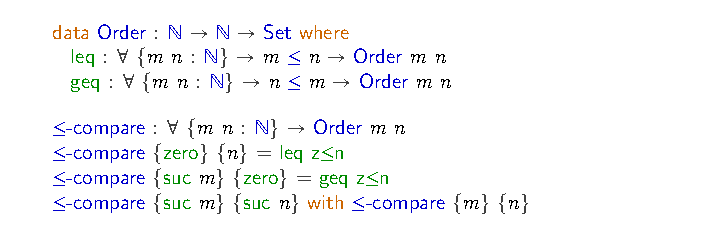
\includegraphics[scale=1.2]{/lib/order_totality.pdf}\]


    % \subsubsection{Other properties}
    % We can show that when a number $n$ is added to a natural number $m$, the result is greater than or equal to $m$. This is defined in Agda as follows:
    % \[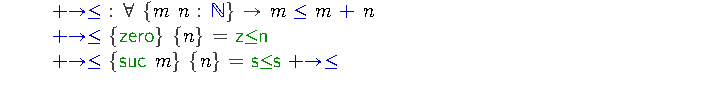
\includegraphics[scale=1.2]{/lib/order_add.pdf}\]


    \subsection{Subtraction} \label{subsec: subtraction}
    In the standard library~\autocite{agda_std}, the subtraction of natural numbers is defined as follows:\footnote{The definition in the standard library directly uses symbol $\mathsf{-}$, but here for clarity we use $\mathsf{\dotdiv}$ instead.}
    \[\includegraphics[scale=1.2]{minus.pdf}\]
    Mathematically we have $ n \dotdiv m = \max(0, n - m)$. This definition is valid and ensures that the result is a natural number. However, there are two problems with this definition for our implementation:
    \begin{itemize}
        \item 
            The definition of $\dotdiv$ is not suitable for this project. Input $n$ should be guaranteed not to be less than $m$, and at any point in the program if there is a subtraction where $n < m$, the program should fail to type check instead of making $0$ type check with it.
        \item
            We do not have many numerical properties of natural numbers that are required for the implementation of the compiler. For example, $n \dotdiv m + m = n$ or $n \dotdiv (n \dotdiv m) = m$ are not guaranteed to hold if we allow $n < m$. 
    \end{itemize}
    A definition of subtraction that ensures the result is a natural number and preserves the numerical properties is required for the implementation of the compiler. The key is to have a proof that the first argument is greater than or equal to the second argument. There are two approaches to achieve this: passing proofs explicitly or using \textsf{Fin}, a dependent type that encodes the proof of boundedness.

    \subsubsection{Explicit proof-passing approach}
    A straightforward approach is directly include a third argument in the subtraction function, which is a proof that the first argument is greater than or equal to the second argument. The definition in Agda is as follows:
    \[\includegraphics[scale=1.2]{/lib/proof/minus.pdf}\]

    The corresponding implementation for subtraction of stack descriptors carries along the proof as follows:
    \[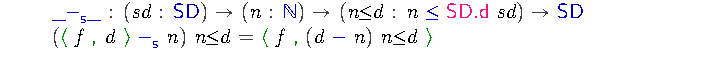
\includegraphics[scale=1.2]{/target/proof/stack_descriptor_minus.pdf}\]

    In the implementation of instruction sequences, we need to carry along the proof as well. The implementation in Agda is as follows:
    \[\includegraphics[scale=1.2]{/target/proof/instruction_dec.pdf}\]

    \subsubsection{\textsf{Fin}-based approach}
    Instead of include the proof directly, we can define the type of the subtrahend to be dependent on the minuend, where the dependence encodes the proof. There is a standard library in Agda on finite sets, where a type $\mb{\mathsf{Fin}}$ is defined as a type that depends on a natural number $n$, where $\mb{\mathsf{Fin}}\ n$ can be seen as the set of natural numbers less than $n$. The definition is as follows:
    \[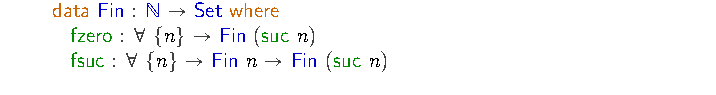
\includegraphics[scale=1.2]{/lib/fin/fin.pdf}\]

    An intuitive explanation of the definition of $\mb{\mathsf{Fin}}$ is as follows:
    \begin{itemize}
        \item Base case: when $n = 0$, we do not have any constructor that gives us an element of type $\mb{\mathsf{Fin}}\ 0$, corresponding to the empty set. 
        \item Inductive case: 
        \begin{figure}[H]
            \centering
            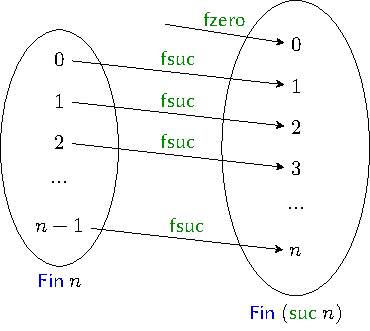
\includegraphics[width=0.5\textwidth]{fin_inductive.pdf}
            \caption{Inductive case of $\mb{\mathsf{Fin}}$}
            \label{fig: fin_inductive}
        \end{figure}
    \end{itemize}

    For subtraction, we only need to change the type of the subtrahend to $\mb{\mathsf{Fin}}\ (\gn{\mathsf{suc}}\ n)$ compared to the implementation of addition. The definition in Agda is as follows:
    \[\includegraphics[scale=1.2]{/lib/fin/minus.pdf}\]

    The corresponding implementation for subtraction of stack descriptors and instruction sequences only requires a change of the type of the subtrahend as follows:
    \[\includegraphics[scale=1.2]{/target/fin/instruction_dec.pdf}\]

    \subsubsection{Comparison of the two approaches}
    The explicit approach carries proofs directly in the type system, which is more transparent but verbose. The $\textsf{Fin}$-based approach initially appears to be more elegant, as it encapsulates bounds check within a refined type. However, this elegance is superficial: constructing a term of type $\mb{\mathsf{Fin}}\ n$ still requires the same underlying proof of boundedness, shifting complexity to auxiliary conversions. 
    
    To prove a property with the $\textsf{Fin}$-based approach, we need the following auxiliary function:
    \[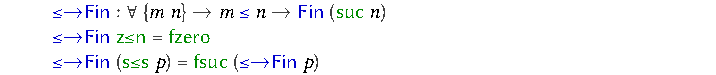
\includegraphics[scale=1.2]{/lib/fin/toFin.pdf}\]

    Here is a comparison of the two approaches representing  $\mathsf{suc}\ (n - m) \equiv \mathsf{suc}\ n - m$:
    \begin{figure}[H]
        \centering
        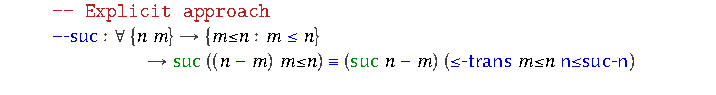
\includegraphics[scale=1.2]{/lib/proof/minus-suc.pdf}
        \includegraphics[scale=1.2]{/lib/fin/minus-suc.pdf}
        \caption{Comparison of explicit vs. \textsf{Fin}-based approaches}
        \label{fig: fin_comparison}
    \end{figure}
    The explicit approach's verbosity pays off in readability when representing properties. the type of the term directly mirrors the mathematical statement with an explicit proof. In contrast, the $\textsf{Fin}$-based approach fractures this relationship, and reconstructing the original subtrahend requires tracing the type of the proof. This becomes cumbersome when the proofs are chained inequalities with transitivity, making the code harder to understand.

    Although the project completed both approaches, the following implementation of the compiler presents the explicit proof-passing approach due to its clarity.

    \subsection{Properties with subtractions} \label{subsec: properties_sub}
    Given the definition of subtraction, the additional properties of natural numbers are summarised in the table below:
    \begin{table}[H]
        \centering
        \begin{tabular}{|l|l|}
            \hline
            \textbf{Agda term} & \textbf{Mathematical meaning} \\
            \hhline{|=|=|}
            \mbt{–-irrelevant} & \makecell{For all $m, n \in \bN$, we consider all terms of $n-m$ \\ with different proofs of $m \leq n$ to be equal.} \\
            \hline
            \mbt{–}\mb{$\to$}\mbt{≤}& $\forall m, n \in \bN.\ m \leq n \Rightarrow m - n \leq m$ \\
            \hline
            \mbt{n–n≡0} & $\forall n \in \bN.\ n - n \equiv 0$ \\
            \hline
            \mbt{–-suc} & $\forall m, n \in \bN.\ \mathsf{suc}\ (n - m) \equiv \mathsf{suc}\ n - m$ \\
            \hline
            \mbt{n–[n–m]≡m} & $\forall m, n \in \bN.\ m \leq n \Rightarrow n - (n - m) \equiv m$ \\
            \hline
            \mbt{n+m–m≡n} & $\forall m, n \in \bN.\ n + m - m \equiv n$ \\
            \hline
            \mbt{suc-d≤d′}\mb{\to}\mbt{d≤d′–[d′–[suc-d]]} & $\forall d, d' \in \bN.\ \textsf{suc } d \leq d' \Rightarrow d \leq d' - (d' - \textsf{suc } d)$ \\
            \hline
        \end{tabular}
        \caption{Properties of natural numbers related to subtraction}
        \label{tab: properties_subtraction}
    \end{table}

    % The equations in the table above are used later in the implementation of the compiler to prove that for instructions with displacement, the given displacement is valid. Here is the mathematical proof of the property $\mb{\mathsf{n\mathord{-}[n\mathord{-}m]\mathord{\equiv}m}}$:
    % \begin{proof}
    %     We need to show that $n - (n - m) \equiv m$ for all $m, n \in \bN$ such that $m \leq n$. We do the following case split:
    %     \begin{itemize}
    %         \item 
    %             If $m = 0$, then the term reduces to $n - n \equiv 0$, which is a term we have already proved.
    %         \item
    %             Otherwise it is guaranteed that $m = \mathsf{suc}\ m'$ for some $m' \in \bN$, and $n = \mathsf{suc}\ n'$ for some $n' \in \bN$, because $m \leq n$. The term reduces to $\mathsf{suc}\ n' - (n' - m') \equiv \mathsf{suc}\ m'$. With congruence, we can reduce the term to $n' - (n' - m') \equiv m'$, which is the inductive hypothesis.
    %     \end{itemize}
    % \end{proof}

    % The implementation of the properties of natural numbers in Agda is as follows:
    % \begin{figure}[H]
    %     \centering
    %     \includegraphics[scale=1.2]{/lib/proof/properties.pdf}
    %     \caption{Properties of natural numbers related to subtraction}
    %     \label{fig: properties_subtraction}
    % \end{figure}


    

    \section{Compiler} \label{sec: compiler}
    This section develops the semantic foundation of the compiler, starting with the presheaf semantics of the target language. Building on this framework, I introduce the continuation-passing constructs to model control flow, enabling a simplified denotational semantics of types and contexts. I then derive a functorial mapping of semantics terms and the target terms. This section concludes with the implementation of the compiler from the denotational semantics of terms in the source language.
    \subsection{Presheaf semantics}
    The denotation semantics interprets types as presheaves over a base category $\Upsigma$. 
    \subsubsection{Base category}
    The base category $\Upsigma$ is specified as follows:
    \begin{itemize}
        \item Objects are stack descriptors ($\textit{sd} = \ang{f, d}$);
        \item Morphisms are stack expansions ($\iota : \textit{sd} \to \textit{sd′}$ for $\textit{sd} \leq_\mathsf{s} \textit{sd′}$).
    \end{itemize}
    We define $\mathsf{SD}$ as the set of stack descriptors. Then the base category is the category determined by preorder $\underline{\mathsf{SD}} = \{\mathsf{SD}, \leq_\mathsf{s}\}$ in Example~\ref{ex: category_preorder}.

    \subsubsection{Semantic category}
    Semantic category $\mathcal{K}$ is the functor category $\text{PDOM}^{\Upsigma^{\textbf{op}}}$, where $\text{PDOM}$ is the category of predomains and continuous functions.
    \begin{itemize}
        \item Objects are presheaves: $P = \Upsigma^{\textbf{op}} \to \text{PDOM}$;
        \item Morphisms are natural transformations: $\eta : P \to Q$ for $P, Q \in \text{PDOM}^{\Upsigma^{\textbf{op}}}$.
    \end{itemize}
    The proof for semantic category is similar to the one in~\secref{sec: ccc_presheaf}, and the full proof is given by Oles in~\autocite{Oles_1, Oles_2}.
    \begin{itemize}
        \item Products are given by pointwise product of presheaves: $P \times Q = \lambda \textit{sd}.\ P\ \textit{sd} \times Q\ \textit{sd}$.
        \item Exponentials $P \Rightarrow_s Q$ are given by the following equation:
                \[\begin{aligned}
                    P \Rightarrow_s Q &= \lambda \textit{sd}.\ \mathcal{K}(\yo (\textit{sd}) \times P, Q) \\
                    &\cong \lambda \textit{sd}.\{F \mid \textit{sd′} \in \Upsigma^{\textbf{op}}, F : (\yo (\textit{sd}) \times P)\ \textit{sd′} \to Q\ \textit{sd′}\} \\
                    &\makebox[0.8\linewidth][r]{\text{by definition of morphisms in Definition~\ref{def: category}}}\\
                    &\cong \lambda \textit{sd}.\{F \mid \textit{sd′} \in \Upsigma^{\textbf{op}}, F : (\Upsigma^{\textbf{op}}(\textit{sd′}, \textit{sd}) \times P)\ \textit{sd′} \to Q\ \textit{sd′}\} \\
                    &\makebox[0.8\linewidth][r]{\text{by definition of $\yo$ in Definition~\ref{def: yoneda}}}\\
                    &\cong \lambda \textit{sd}.\{F \mid \textit{sd′} \in \Upsigma, F : (\Upsigma(\textit{sd}, \textit{sd′}) \times P)\ \textit{sd′} \to Q\ \textit{sd′}\} \\
                    &\makebox[0.8\linewidth][r]{\text{by definition of opposite category in Definition~\ref{def: opposite}}}\\
                    &\cong \lambda \textit{sd}.\{F \mid \textit{sd′} \in \Upsigma, F : \textit{sd} \leq_\mathsf{s} \textit{sd′} \to P\ \textit{sd′} \to Q\ \textit{sd′}\} \\
                    &\makebox[0.8\linewidth][r]{\text{by definition of $\Upsigma$ above}}\\
                \end{aligned}\]
    \end{itemize}
    
    The definition of products and exponentials in Agda is as follows:
    \[\includegraphics[scale=1.2]{/compiler/product_exponentials.pdf}\]

    The definition of exponentials captures the essence of stack-respecting computations in the compiler. 
    \begin{itemize}
        \item $\textit{sd} \leq_\mathsf{s} \textit{sd′}$ means the new stack descriptor $\textit{sd′}$ is larger than the old stack descriptor $\textit{sd}$, representing the dynamic expansion of the stack during execution.

        \item $P$ and $Q$ are denotational semantics of types. 
    \end{itemize}
    The exponential $P \Rightarrow_\textsf{s} Q$ is a function that given a proof of stack growth, transforming a $P$-value at $\textit{sd′}$ into a $Q$-value at $\textit{sd′}$, and the $\forall{\textit{sd′}}$ quantifier guarantees it works no matter how the stack grows. It is designed in this way so that a functor $\intp{-} : \Theta \to \mathcal{K}$ exists that interprets the type constructor $\Rightarrow$ as the exponential functor $\Rightarrow_s$.

    \subsection{Continuations}
    In Reynolds' model, we construct $\mathsf{Compl}$ and $\mathsf{Intcompl}$\footnote{In the work of Reynolds, $\mathsf{compl}$ and $\mathsf{intcompl}$ are introduced as new types in the source language, and the definitions here are the denotational semantics of those types, respectively. Since these two introduced types are only used for the denotational semantics, I think directly defining them as denotational semantics constructs is natural and sufficient.} as tools in the denotational semantics to represent command continuations and integer continuations, respectively. We can think of integer continuations as a function that takes an integer and returns a command continuation. Mathematically we have
    \[\mathsf{Compl}\ \textit{sd} : \mathsf{SD} \to O \qquad \mathsf{Intcompl}\ \textit{sd} : \bZ \to (\mathsf{SD} \to O)\]
    where $O$ is an unspecified domain of outputs.

    For code generation I define the continuation to be the instruction sequence in the target language:
    \[\mathsf{Compl}\ \textit{sd} = \textsf{I}_{\textit{sd}}\]

    The definition of integer continuation is an exponential object in the presheaf category, which is defined as follows:
    \[\mathsf{Intcompl} = R \Rightarrow_s \mathsf{Compl} \]
    where $R$ is the functor corresponding to the right-hand sides in the target language, $R\ \textit{sd} = \textsf{R}_{\textit{sd}}$. This works because the right-hand sides are all integer expressions we can use according to the grammar of the target language. The functorial mapping is defined later in~\secref{subsec: functorial_mapping}.
    
    Thus we can directly use the definition of $R$ in the target language to define the integer continuation as follows:
    \[\includegraphics[scale=1.2]{/compiler/continuations.pdf}\]

    \subsection{Denotational semantics of types and contexts} \label{subsec: type_interpretation}
    With the idea of continuation, the denotational semantics of types can be defined as follows:
    \begin{itemize}
        \item Command passes on command continuations;
        \item Integer expressions takes an integer continuation and returns a command continuation;
        \item Integer acceptors take a command continuation and returns an integer continuation;
        \item Integer variables can be used both as an integer expression and an integer acceptor, so it has the denotational semantics of both, defined as a product of the two.
    \end{itemize}
    
    The denotational semantics of types in Agda as follows:
    \[\includegraphics[scale=1.2]{/compiler/type_interpretation.pdf}\]

    The denotational semantics of contexts is essentially a list expressed by the product of the denotational semantics of the types in the context. The denotational semantics of contexts is defined as follows, where we use \mb{∅} to denote the denotational semantics of the empty context:
    \[\includegraphics[scale=1.2]{/compiler/context_interpretation.pdf}\]

    \subsection{Functorial mapping} \label{subsec: functorial_mapping}
    The denotational semantics of terms is defined as a functor. Before we define its object mapping, we need to define the functorial mapping, which acts on the morphisms of the base category $\Upsigma$. 

    Since the morphisms of the base category $\Upsigma$ are stack expansions, the functorial mapping essentially lifts a semantic object indexed by a stack descriptor $\textit{sd}$ to a semantic object indexed by a larger stack descriptor $\textit{sd′}$. This ensures the denotational semantics of terms remains valid when the stack grows.

    Functorial mapping for exponentials is simple, as the exponential \textit{P} $\mathsf{\Rightarrow_\textsf{S}}$ \textit{Q} \textit{sd} can transforms a $P$-value at any $\textit{sd′}$ greater than $\textit{sd}$ into a $Q$-value at $\textit{sd′}$. To construct a new exponential of type $\mathsf{P \Rightarrow_\textsf{S} Q\ \textit{sd′}}$, we simply take a new $P$-value at $\textit{sd″}$ which is greater than $\textit{sd′}$, and use the original exponential to transform it into a $Q$-value at $\textit{sd′}$, as $\textit{sd″}$ is guaranteed to be greater than $\textit{sd}$ due to the transitivity of order of the stack descriptors. 

    Functorial mapping for types can be defined based on functorial mapping of exponentials and products (defined point-wise), as denotational semantics of types is defined as either product or exponential. As a list of types, the functorial mapping of contexts is simply a map of the functorial mapping of types in the list. The definition of functorial mapping in Agda is as follows:
    \[\includegraphics[scale=1.2]{/compiler/fmap_ctx.pdf}\]

    Similarly, we can use transitivity of order to define the functorial mapping of the denotational semantics of left-hand sides, as the definition of left-hand sides requires a proof. Since simple right-hand sides are defined from left-hand sides and literals, we can use the functorial mapping of left-hand sides to define the functorial mapping of simple right-hand sides. The functorial mapping of the denotational semantics of left-hand sides and simple right-hand sides is defined as follows:
    \[\includegraphics[scale=1.2]{/compiler/fmap_LS.pdf}\]
    Similarly, the functorial mapping of right-hand sides can be defined based on the functorial mapping of simple right-hand sides. Since it is not used in the implementation of the compiler, the definition is omitted here.

    \subsubsection[Functorial mapping for instruction sequences]{Functorial mapping for instruction sequences}
    The functorial mapping of the denotational semantics of instruction sequences is defined as follows, assuming the stack descriptor $\textit{sd′} = \ang{f',d'}$ is greater than $\textit{sd} = \ang{f,d}$:
    \begin{itemize}
        \item When $f < f'$, we use the $\mathsf{popto}$ instruction that directly pops the stack to $\textit{sd}$;
        \item When $f' = f$ and $d < d'$, we use $\mathsf{adjustdisp}$ to decrease the displacement by $d'-d$.
    \end{itemize}
    In the Agda implementation, we also need to show that after the the adjustment, the stack descriptor is now $\textit{sd}$. This requires the term $\mb{\mathsf{n\mathord{-}[n\mathord{-}m]\mathord{\equiv}m}}$ proved in~\secref{subsec: properties_sub}. The functorial mapping of the denotational semantics of instruction sequences is defined as follows:
    \[\includegraphics[scale=1.2]{/compiler/fmap_instruction.pdf}\]

    \subsection{Compilation}
    The denotational semantics of terms is defined as a morphism from the denotational semantics of contexts to the denotational semantics of types. The denotational semantics of terms is a functor from the source language to the target language, which directly yields a compiler. Similarly, it is a family of continuous functions indexed by the stack descriptor. The denotational semantics of terms has the following type in Agda:
    \[\includegraphics[scale=1.2]{/compiler/term_interpretation_type.pdf}\]

    The denotational semantics of the terms corresponding to all rules in the typing judgement mentioned in~\secref{subsec: terms} is defined as follows: 

        \subsubsection{Variables}
        We define an auxiliary function that simply gets the variable from the list of variables (the context), and the denotational semantics of variables is given by applying this function:
        \[\includegraphics[scale=1.2]{/compiler/term_var.pdf}\]

        \subsubsection{Subtyping}
        The idea of subtyping is to use a term of type $A$ as a term of type $A'$, where $A$ is a subtype of $A'$. We define an auxiliary function that takes in the subtype relation $A\leq:A'$ and the denotational semantics of $A$, and returns the denotational semantics of $A'$. 
        \begin{itemize}
            \item For \gnt{var-≤:-exp} and \gnt{⟦var-≤:-acc}, sincethe denotational semantics of integer variable is defined as product of the denotational semantics of integer expression and integer acceptor in~\secref{subsec: type_interpretation}, we can simply use the projection to get the denotational semantics of either side.
            \item For \gnt{≤:-refl}, we can simply use the identity function.
            \item For \gnt{≤:-trans}, we can use the composition of the two functions.
            \item For \gnt{≤:-fn}, we can use a contravariant function.
        \end{itemize}
        The denotational semantics of subtyping is given by applying the auxiliary function:
        \[\includegraphics[scale=1.2]{/compiler/term_subtype.pdf}\]

        \subsubsection{Lambda abstraction}
        \begin{itemize}
            \item For lambda, we need to extend the context $\gamma$ with the extra variable in the lambda term. This is done by using the functorial mapping of the denotational semantics of contexts.
            \item For application, we simply apply the denotational semantics of the lambda term to the denotational semantics of the argument, where the proof is simply the reflexivity of the order of stack descriptors.
        \end{itemize}
        The denotational semantics of lambda abstraction is defined as follows:
        \[\includegraphics[scale=1.2]{/compiler/term_lambda.pdf}\]

        \subsubsection{Command}
        \begin{itemize}
            \item For skip, we simply return the continuation $\kappa$ without changing it.
            \item For sequence, we need to prefix the continuation with the denotational semantics of the second command, and then prefix it with the denotational semantics of the first command, as the continuation $\kappa$ is to be performed after both commands.
            \item For assignment, the definition is similar to sequence, as we need to prefix the continuation with the denotational semantics of the integer accepter and then prefix it with the denotational semantics of the integer expression.
        \end{itemize}
        The denotational semantics of commands is defined as follows:
        \[\includegraphics[scale=1.2]{/compiler/term_comm.pdf}\]

        \paragraph{New variable}
        The denotational semantics of \gnt{NewVar} command is more complicated. We prefix the continuation with the following in order:
        \begin{enumerate}
            \item an assignment with displacement adjustment $1$, representing the new variable;
            \item the denotational semantics of the command where this variable is used;
            \item an adjustment of the stack descriptor by $-1$, which deallocates the new variable.
        \end{enumerate}
        In step 2, the denotational semantics of the command in \textsf{NewVar} needs to be applied to
        \begin{itemize}
            \item a stack descriptor increased by $1$ to include the new variable;
            \item an extended denotational semantics of the context, which includes the new variable.
        \end{itemize}
        The denotational semantics of the new variable is a product of the denotational semantics of an integer expression and the denotational semantics of an integer acceptor by definition in~\secref{subsec: type_interpretation}.
        \begin{itemize}
            \item The expression component fills the a given integer continuation $\beta$ with the stack descriptor for the new variable;
            \item The acceptor component prefixes the continuation $\kappa$ with an assignment of the new variable.
        \end{itemize}

        Please see Appendix~[TBD] for the full implementation of the function \textsf{NewVar}.

        \subsubsection{Integer expression} \label{subsubsec: compiler_intexp}
        The denotational semantics of type $\mathsf{intexp}$ is an exponential from an integer continuation to a command continuation. We need to fill the integer continuation with appropriate $R$ terms to get the command continuation. 
        \begin{itemize}
            \item For integer literals, we can simply fill in the integer literal (as an $\mathsf{R}$ term) to the integer continuation $\beta$.
            \item For addition and negation, we wish to fill the negation or the sum of the given expression(s) to the integer continuation $\beta$. However, this is only possible when the given expression(s) are simple left-hand sides, as the grammar of the target language in Figure~\ref{fig: target_grammar} restricts right-hand sides to contain at most one operator. An auxiliary function \textsf{use-temp} that stores the intermediate result of given expressions is introduced to solve this problem. 
        \end{itemize}
        With \textsf{use-temp}, the denotational semantics of addition and negation is simply wrapping $\beta$ with a lambda function using \textsf{use-temp} to get temporary variable(s) of the given expression(s), and directly fill the negation or the sum of the variable(s) to the integer continuation $\beta$. Note that in the denotational semantics of addition, we need to use the functorial mapping of simple right-hand sides for the first argument, as the stack may grow during the evaluation of the second argument. The denotational semantics of integer expressions is defined as follows:
        \[\includegraphics[scale=1.2]{/compiler/term_intexp.pdf}\]
        The auxiliary function \textsf{use-temp} checks if the given expression is a simple left-hand side,
        \begin{itemize}
            \item If it is, we simply fill the expression to the integer continuation $\beta$.\footnote{The type of $\beta$ here is actually a bit different to integer continuation I defined, as it only accepts simple right-hand sides instead of right-hand sides. Reynolds gave a wrong definition of the type of this term. I have corrected it in my Agda implementation.}
            \item If it is not, we need to use a temporary variable to store the result of the expression, and then fill the temporary variable to the integer continuation $\beta$.
        \end{itemize}
        However, regarding the stack descriptor, according to Reynolds' model, we assume
        \begin{itemize}
            \item \textit{sd} is the stack descriptor before the evaluation of plus or negation, which is the position of the temporary variable in the stack.
            \item \textit{sd′} is the stack descriptor after the evaluation on the given expression and just before the assignment of the temporary variable. \textit{sd} ≤ₛ \textit{sd′} is guaranteed.
            \item \textit{sd″} = \textit{sd} +ₛ 1 is the stack descriptor after the assignment of the temporary variable, as it is just large enough to hold the temporary variable.
        \end{itemize}
        In Reynolds' model, the stack descriptor can be directly adjusted from \textit{sd′} to \textit{sd″}. However, in the Agda implementation, we need to know whether the adjustment is positive or negative and use \textsf{assign-inc} or \textsf{assign-dec} respectively. This is done by using \mbt{≤-compare} in Table~\ref{tab: properties}. We also need to show that the adjustment is valid for each case. Please refer to Appendix~[TBD] for the full implementation of the function \textsf{use-temp}.
        % The auxiliary function \textsf{use-temp} is defined as follows:
        % \[\includegraphics[scale=1.2]{/compiler/assign_use-temp.pdf}\]
        

        \subsubsection{Compilation for closed program} \label{subsubsec: compilation}
        To define a compilation function for closed programs in the source language, we use the denotational semantics of terms and fill in the initial stack descriptor ($\ang{0, 0}$), the empty context (\textsf{unit}), a trivial proof for stack descriptor being not less than itself (\textsf{≤ₛ-refl}) and the continuation representing the last instruction (\textsf{stop}):
        \[\includegraphics[scale=1.2]{/compiler/compilation.pdf}\]




\chapter{Evaluation}
    \minitoc
    This chapter evaluates the implementation with integration tests and a feature checklist and then discusses the success criteria of the project.
    \section{Tests}
    The best way to evaluate a formalised compiler project is to formalise compiler correctness, which requires the full definition of the operational semantics of the source language and the target language, and then prove that for any program $e$ in the source language and the program $e'$ it compiles to in the target language, the value $v'$ that $e'$ evaluates to is also the compilation of the value $v$ that $e$ evaluates to. Due to time limitations, this is beyond the scope of this project. Instead, I used a set of integration tests that covers all features of the source language and the target language to evaluate the correctness of the compiler. All of the test cases have been passed successfully.

    \subsection{Test cases}
    Each test case is an Agda program defined with the follow syntax, where \gn{\textsf{Skip}} is replaced with any closed program in the source language and \gn{\textsf{stop}} is replaced with the expected compiled result in the target language:
    \begin{figure}[H]
        \centering
        \includegraphics[scale=1.2]{/test/example.pdf}
        \caption{Test 0 as an example of test cases}
        \label{fig: test_case_0}
    \end{figure}
    where definition of the \mb{\textsf{compile-closed}} function is specified in~\secref{subsubsec: compilation}. Each test case type checks only if both the source term and target term are well-typed, and the compiled result of the source term is definitionally equal to the target term.

    There are special tests to check that some expressions in the source language compiles to the same expression in the target language. Such test is defined as follows:
    \begin{figure}[H]
        \centering
        \includegraphics[scale=1.2]{/test/equivalence.pdf}
        \caption{Test 3′ as an example for checking equivalent compiled results}
        \label{fig: test_case_3′}
    \end{figure}

    The full test cases are available in the appendix [TBD]. Here is a summary of the test cases:
    % \begin{enumerate}[label=\textbf{Test \arabic*.}, leftmargin=*]
    %     \setcounter{enumi}{-1}
    %     \item $\mathsf{skip}$
    %     \item $\mathsf{x := 2}$
    %     \item $\mathsf{x := (\mathnormal{\lambda} a.\ a)\ 4}$
    %     \item $\mathsf{x := (\mathnormal{\lambda} a.\ (\mathnormal{\lambda} b.\ a+b)\ 2)\ 3}$
    %     \item[\textbf{Test 3′.}] $\mathsf{x := 3 + 2}$
    %     \item $\mathsf{x := -3;\ y := (\mathnormal{\lambda} a. x)\ 2}$
    %     \item $\mathsf{x := 2;\ x := x + 1}$
    %     \item[\textbf{Test 5′.}] $\mathsf{x := 2;\ skip;\ x := x + 1}$
    %     \item $\mathsf{x := 2;\ x := -x + 1}$
    %     \item $\mathsf{x := (\mathnormal{\lambda} a.\ -a+1)\ 2}$
    % \end{enumerate}
    \begin{table}[H]
        \centering
        \begin{tabular}{| c | c |}
            \hline
            \textbf{Test case} & \textbf{Source term} \\
            \hhline{|=|=|}
            \textbf{Test 0} & $\mathsf{skip}$ \\
            \hline
            \textbf{Test 1} & $\mathsf{x := 2}$ \\
            \hline
            \textbf{Test 2} & $\mathsf{x := (\mathnormal{\lambda} a.\ a)\ 4}$ \\
            \hline
            \textbf{Test 3} & $\mathsf{x := (\mathnormal{\lambda} a.\ (\mathnormal{\lambda} b.\ a+b)\ 2)\ 3}$ \\
            \hline
            \textbf{Test 3′} & $\mathsf{x := 3 + 2}$ \\
            \hline
            \textbf{Test 4} & $\mathsf{x := -3;\ y := (\mathnormal{\lambda} a. x)\ 2}$ \\
            \hline
            \textbf{Test 5} & $\mathsf{x := 2;\ x := x + 1}$ \\
            \hline
            \textbf{Test 5′} & $\mathsf{x := 2;\ skip;\ x := x + 1}$ \\
            \hline
            \textbf{Test 6} & $\mathsf{x := 2;\ x := -x + 1}$ \\
            \hline
            \textbf{Test 7} & $\mathsf{x := (\mathnormal{\lambda} a.\ -a+1)\ 2}$ \\
            \hline
        \end{tabular}
        \caption{Test cases}
        \label{tab: test_cases}
    \end{table}
    where \textbf{Test 3} and \textbf{Test 3′}, \textbf{Test 5} and \textbf{Test 5′} compile to the same target term. 
    
    \textbf{Test 3} and \textbf{Test 3′} are equivalent in terms of compilation because the compilation directly substitutes the value in corresponding lambda terms. 
    
    \textbf{Test 5} and \textbf{Test 5′} are equivalent in terms of compilation because $\mathsf{skip}$ is a no-op in the source language.

    \subsection{Feature checklist}
    Traditional unit tests are not suitable for this project, as many typing judgement rules cannot be tested in isolation. For example, testing subtyping rule (Figure~\ref{fig: rule_subtype}) or any of the integer expression typing rules (Figure~\ref{fig: rule_intexp}) inherently requires embedding them in a well-typed command (\textsc{NewVar} in Figure~\ref{fig: rule_comm_2}), as the compiler only accepts complete commands. 

    Instead, I employed integration testing with a feature checklist, ensuring comprehensive coverage by validating all typing rules and targeting edge cases.
    \begin{table}[H]
        \centering
        \begin{tabular}{| c | c | c | c |}
            \hline
            \textbf{Feature}  & \textbf{Typing judgement} & \textbf{Specification} & \textbf{Test cases} \\
            \hhline{|=|=|=|=|}
            Variable & \textsc{Var} & - & 1, 2, 3, 3′, 4, 5, 5′, 6, 7 \\ \cline{3-4}
            \hline
            \multirow{2}{*}{Subtyping} 
                & \multirow{2}{*}{\textsc{Sub}} 
                    & \textsf{intvar} $\leq:$ \textsf{intacc} & 1, 2, 3, 3′, 4, 5, 5′, 6, 7  \\ \cline{3-4}
                &   & \textsf{intvar} $\leq:$ \textsf{intexp} & 4, 5, 5′, 6 \\
            \hline
            \multirowcell{4}{Lambda\\abstraction} 
                & \multirow{3}{*}{\textsc{Lambda}} 
                    & - & 2, 3, 4, 7 \\ \cline{3-4}
                &   & Multiple variables & 3  \\ \cline{3-4}
                &   & Free variables & 4 \\ \cline{2-4}
                & \textsc{App} & - & 2, 3, 4, 7  \\
            \hline
            \multirow{7}{*}{Command} 
                & \textsc{Skip} & - & 0, 5′ \\ \cline{2-4}
                & \multirow{2}{*}{\textsc{Seq}} 
                    & - & 4, 5, 5′, 6 \\ \cline{3-4}
                &   & Multiple sequencing & 5′ \\ \cline{2-4}
                & \multirow{2}{*}{\textsc{NewVar}} 
                    & - & 1, 2, 3, 3′, 4, 5, 5′, 6, 7 \\ \cline{3-4}
                &   & Multiple variables & 4 \\ \cline{2-4}
                & \multirow{2}{*}{\textsc{Assign}} 
                    & -  & 1, 2, 3, 3′, 4, 5, 5′, 6, 7  \\ \cline{3-4}
                &   & Self-referential assignments & 5, 5′, 6 \\
            \hline
            \multirowcell{5}{Integer\\expression} 
                & \multirow{2}{*}{\textsc{Lit}}  
                    & Natural number  & 1, 3, 3′, 4, 5, 6, 7 \\ \cline{3-4}
                &   & Negative number & 2, 4 \\ \cline{2-4}
                & \textsc{Neg} & - & 5, 5′, 6, 7  \\ \cline{2-4}
                & \textsc{Plus} & - & 3, 3′, 6, 7  \\ \cline{2-4}
                & -             & Multiple expressions & 6, 7 \\
            \hline
        \end{tabular}

        \caption{Feature checklist}
        \label{tab: feature_checklist}
    \end{table}

    The specifications that include multiple variables, free variables and self-referential assignments ensure that the translation of the Debrujin index of the context works correctly under edge cases.

    The specification of multiple expressions in integer expression is necessary because the target language does not support doing multiple integer operations in a single instruction, as specified in Figure~\ref{fig: target_grammar}. As a result, special tests are required to check that the compiler correctly translates integer expressions with multiple operations into a continuation of single operations defined in the target language. 

    The feature checklist covers all the typing rules in the source language, including edge cases including multiple variables, free variables and self-referential assignments. Additionally, I account for target-language-specific constraints, ensuring multiple operations are translated into simple instructions with continuation. The tests cover all the cases in the feature checklist, ensuring that the compiler generates expected target code under all circumstances.

    \section{Extensibility}
    This project is inherently extensible, as all of the components are defined as terms and types in Agda. The compiler can be extended to support more features by adding new terms in the form of type judgement rules in the source language, adding any new instructions in the target language if needed, and write corresponding compilation rules.

    \section{Success criteria}
    The project has met the success criteria as follows:
    \begin{itemize}
        \item
            A formalisation of the source language has been given in Agda, which includes the syntax, typing rules and operational semantics. 

        \item
            A formalisation of the target language has been given in Agda, which includes all instructions from the instruction set. Rigorous definitions of the operation of the stack descriptors are given, ensuring correctness and preserving the mathematical properties of the stack descriptors.
        
        \item
            A formalisation of the compiler has been given in Agda, which includes the denotational semantics of the source language and a term for compilation.

        \item 
            Integration tests have been given in Agda, which cover all the case in the feature checklist. The tests ensure that the compiler generates expected target code under all circumstances.
    \end{itemize}

    The following are the extension criteria that are met:
    \begin{itemize}
        \item 
            A customised library have been developed, which includes rigorous definitions of subtraction of natural numbers and corresponding properties. Two approaches to rigorous definition of subtraction has been implemented and compared.
        \item
            Operational semantics of the source language has been defined with renaming, substitution and reduction rules.
        \item
            Complicated functions defined for translating expressions with multiple operations in the source language to a continuation of simple instructions in the target language. 

    \end{itemize}

\chapter{Conclusion}
    \minitoc
    \section{Results}
    This project has successfully implemented a compiler from a source language (STLC with store) to a target language (stack machine) in Agda. The compiler is defined as a functor from the source language to the target language, which is directly generated from the denotational semantics of the source language. The compiler validates and refines Reynolds' theory~\autocite{Reynolds}, offers a concrete example of how category-theoretic semantics can generate intermediate code.

    \section{Lessons learned}
    The project has been quite challenging as I have to learn both category theory and Agda from scratch, and apply them to implementation. The implementation process revealed unexpected gaps between Reynolds' theoretical framework and the computational realisation: while his denotational semantics provided core definitions, actualising them in Agda required formalising numbers, their operations, and properties and diagnosing and resolving type mismatches and ambiguities in the original paper~\autocite{Reynolds}. These hurdles highlighted how even meticulously defined theories can be complicated when translated to working systems.


    In terms of planning the project, the project has deviated slightly from the original timetable in the project proposal due to differences
    between the anticipated structure of the project and its actual development process. When I was drafting the proposal, I expected the workflow to be similar to a standard compiler, so I divided the work into components including basic instructions, variable declarations and conditionals, allocating two weeks for each. In hindsight, these components are similar term definitions, while the core of the project can be more accurately divided into three main tasks: defining the source language, defining the target language, and defining the translation between the two. The most time-consuming aspect of each step has been understanding their formal definitions in the paper and addressing the missing details in the Agda implementation.

    Overall, the project has been a valuable learning experience, and I have gained a deeper understanding of both Category Theory and Agda and an exciting glimpse of how the correspondences between logic, type theory and category theory can be used to implement a compiler.


    \section{Future work}
    The project has successfully implemented the compiler, but there are still many areas for improvement and further research:
    \begin{itemize}
        \item 
            The compiler can be extended to support more features from Reynolds' paper~\autocite{Reynolds}, such as subroutines and iterations.
        \item
            The operational semantics of the target language can be defined, which can be used, along with the operational semantics of the source language, to prove the correctness of the compiler.
        \item
            Reynolds pointed out that the requirement of instructions being natural transformation must be relaxed to allow for instruction sequences that differ operationally but are equivalent in terms of denotational semantics~\autocite[Ch. 6]{Reynolds}. Extra research can be done to develop a reasonable equational theory that can be stated directly on the instruction sequences, under which the semantics actually becomes a true functor category model (i.e. naturality holds).
    \end{itemize}

\printbibliography

\appendix

\chapter{Operational Semantics of the source language} \label{app: operational_semantics}
    \minitoc
    The operational semantics of the source language is defined with renaming, substitution and reduction rules. The implementation is as follows:
    \begin{figure}[H]
        \centering
        \includegraphics[scale=1.2]{/source/operational_semantics_1.pdf}
        \caption{Operational semantics of the source language (Part 1)}
        \label{fig: operational_semantics_1}
    \end{figure}
    \begin{figure}[H]
        \centering
        \includegraphics[scale=1.2]{/source/operational_semantics_2.pdf}
        \caption{Operational semantics of the source language (Part 2)}
        \label{fig: operational_semantics_2}
    \end{figure}


\cleardoublepage
\let\cleardoublepage\clearpage
\pagestyle{empty}
\pagenumbering{gobble}
\includepdf[pages=-, fitpaper=true, pagecommand={}]{final_proposal.pdf}
\AtBeginShipoutNext{\AtBeginShipoutDiscard}
\end{document}